\documentclass[1p]{elsarticle_modified}
%\bibliographystyle{elsarticle-num}

%\usepackage[colorlinks]{hyperref}
%\usepackage{abbrmath_seonhwa} %\Abb, \Ascr, \Acal ,\Abf, \Afrak
\usepackage{amsfonts}
\usepackage{amssymb}
\usepackage{amsmath}
\usepackage{amsthm}
\usepackage{scalefnt}
\usepackage{amsbsy}
\usepackage{kotex}
\usepackage{caption}
\usepackage{subfig}
\usepackage{color}
\usepackage{graphicx}
\usepackage{xcolor} %% white, black, red, green, blue, cyan, magenta, yellow
\usepackage{float}
\usepackage{setspace}
\usepackage{hyperref}

\usepackage{tikz}
\usetikzlibrary{arrows}

\usepackage{multirow}
\usepackage{array} % fixed length table
\usepackage{hhline}

%%%%%%%%%%%%%%%%%%%%%
\makeatletter
\renewcommand*\env@matrix[1][\arraystretch]{%
	\edef\arraystretch{#1}%
	\hskip -\arraycolsep
	\let\@ifnextchar\new@ifnextchar
	\array{*\c@MaxMatrixCols c}}
\makeatother %https://tex.stackexchange.com/questions/14071/how-can-i-increase-the-line-spacing-in-a-matrix
%%%%%%%%%%%%%%%

\usepackage[normalem]{ulem}

\newcommand{\msout}[1]{\ifmmode\text{\sout{\ensuremath{#1}}}\else\sout{#1}\fi}
%SOURCE: \msout is \stkout macro in https://tex.stackexchange.com/questions/20609/strikeout-in-math-mode

\newcommand{\cancel}[1]{
	\ifmmode
	{\color{red}\msout{#1}}
	\else
	{\color{red}\sout{#1}}
	\fi
}

\newcommand{\add}[1]{
	{\color{blue}\uwave{#1}}
}

\newcommand{\replace}[2]{
	\ifmmode
	{\color{red}\msout{#1}}{\color{blue}\uwave{#2}}
	\else
	{\color{red}\sout{#1}}{\color{blue}\uwave{#2}}
	\fi
}

\newcommand{\Sol}{\mathcal{S}} %segment
\newcommand{\D}{D} %diagram
\newcommand{\A}{\mathcal{A}} %arc


%%%%%%%%%%%%%%%%%%%%%%%%%%%%%5 test

\def\sl{\operatorname{\textup{SL}}(2,\Cbb)}
\def\psl{\operatorname{\textup{PSL}}(2,\Cbb)}
\def\quan{\mkern 1mu \triangleright \mkern 1mu}

\theoremstyle{definition}
\newtheorem{thm}{Theorem}[section]
\newtheorem{prop}[thm]{Proposition}
\newtheorem{lem}[thm]{Lemma}
\newtheorem{ques}[thm]{Question}
\newtheorem{cor}[thm]{Corollary}
\newtheorem{defn}[thm]{Definition}
\newtheorem{exam}[thm]{Example}
\newtheorem{rmk}[thm]{Remark}
\newtheorem{alg}[thm]{Algorithm}

\newcommand{\I}{\sqrt{-1}}
\begin{document}

%\begin{frontmatter}
%
%\title{Boundary parabolic representations of knots up to 8 crossings}
%
%%% Group authors per affiliation:
%\author{Yunhi Cho} 
%\address{Department of Mathematics, University of Seoul, Seoul, Korea}
%\ead{yhcho@uos.ac.kr}
%
%
%\author{Seonhwa Kim} %\fnref{s_kim}}
%\address{Center for Geometry and Physics, Institute for Basic Science, Pohang, 37673, Korea}
%\ead{ryeona17@ibs.re.kr}
%
%\author{Hyuk Kim}
%\address{Department of Mathematical Sciences, Seoul National University, Seoul 08826, Korea}
%\ead{hyukkim@snu.ac.kr}
%
%\author{Seokbeom Yoon}
%\address{Department of Mathematical Sciences, Seoul National University, Seoul, 08826,  Korea}
%\ead{sbyoon15@snu.ac.kr}
%
%\begin{abstract}
%We find all boundary parabolic representation of knots up to 8 crossings.
%
%\end{abstract}
%\begin{keyword}
%    \MSC[2010] 57M25 
%\end{keyword}
%
%\end{frontmatter}

%\linenumbers
%\tableofcontents
%
\newcommand\colored[1]{\textcolor{white}{\rule[-0.35ex]{0.8em}{1.4ex}}\kern-0.8em\color{red} #1}%
%\newcommand\colored[1]{\textcolor{white}{ #1}\kern-2.17ex	\textcolor{white}{ #1}\kern-1.81ex	\textcolor{white}{ #1}\kern-2.15ex\color{red}#1	}

{\Large $\underline{12a_{1248}~(K12a_{1248})}$}

\setlength{\tabcolsep}{10pt}
\renewcommand{\arraystretch}{1.6}
\vspace{1cm}\begin{tabular}{m{100pt}>{\centering\arraybackslash}m{274pt}}
\multirow{5}{120pt}{
	\centering
	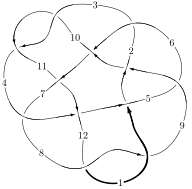
\includegraphics[width=112pt]{../../../GIT/diagram.site/Diagrams/png/2049_12a_1248.png}\\
\ \ \ A knot diagram\footnotemark}&
\allowdisplaybreaks
\textbf{Linearized knot diagam} \\
\cline{2-2}
 &
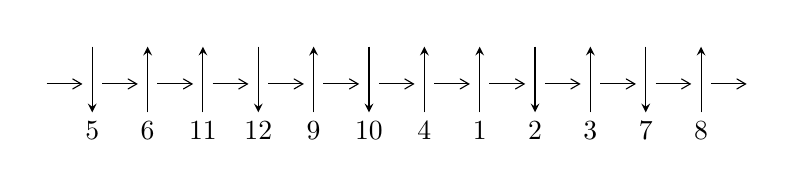
\begin{tikzpicture}[x=20pt, y=17pt]
	% nodes
	\node (C0) at (0, 0) {};
	\node (C1) at (1, 0) {};
	\node (C1U) at (1, +1) {};
	\node (C1D) at (1, -1) {5};

	\node (C2) at (2, 0) {};
	\node (C2U) at (2, +1) {};
	\node (C2D) at (2, -1) {6};

	\node (C3) at (3, 0) {};
	\node (C3U) at (3, +1) {};
	\node (C3D) at (3, -1) {11};

	\node (C4) at (4, 0) {};
	\node (C4U) at (4, +1) {};
	\node (C4D) at (4, -1) {12};

	\node (C5) at (5, 0) {};
	\node (C5U) at (5, +1) {};
	\node (C5D) at (5, -1) {9};

	\node (C6) at (6, 0) {};
	\node (C6U) at (6, +1) {};
	\node (C6D) at (6, -1) {10};

	\node (C7) at (7, 0) {};
	\node (C7U) at (7, +1) {};
	\node (C7D) at (7, -1) {4};

	\node (C8) at (8, 0) {};
	\node (C8U) at (8, +1) {};
	\node (C8D) at (8, -1) {1};

	\node (C9) at (9, 0) {};
	\node (C9U) at (9, +1) {};
	\node (C9D) at (9, -1) {2};

	\node (C10) at (10, 0) {};
	\node (C10U) at (10, +1) {};
	\node (C10D) at (10, -1) {3};

	\node (C11) at (11, 0) {};
	\node (C11U) at (11, +1) {};
	\node (C11D) at (11, -1) {7};

	\node (C12) at (12, 0) {};
	\node (C12U) at (12, +1) {};
	\node (C12D) at (12, -1) {8};
	\node (C13) at (13, 0) {};

	% arrows
	\draw[->,>={angle 60}]
	(C0) edge (C1) (C1) edge (C2) (C2) edge (C3) (C3) edge (C4) (C4) edge (C5) (C5) edge (C6) (C6) edge (C7) (C7) edge (C8) (C8) edge (C9) (C9) edge (C10) (C10) edge (C11) (C11) edge (C12) (C12) edge (C13) ;	\draw[->,>=stealth]
	(C1U) edge (C1D) (C2D) edge (C2U) (C3D) edge (C3U) (C4U) edge (C4D) (C5D) edge (C5U) (C6U) edge (C6D) (C7D) edge (C7U) (C8D) edge (C8U) (C9U) edge (C9D) (C10D) edge (C10U) (C11U) edge (C11D) (C12D) edge (C12U) ;
	\end{tikzpicture} \\
\hhline{~~} \\& 
\textbf{Solving Sequence} \\ \cline{2-2} 
 &
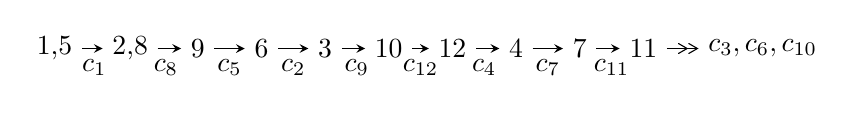
\begin{tikzpicture}[x=23pt, y=7pt]
	% node
	\node (A0) at (-1/8, 0) {1,5};
	\node (A1) at (17/16, 0) {2,8};
	\node (A2) at (17/8, 0) {9};
	\node (A3) at (25/8, 0) {6};
	\node (A4) at (33/8, 0) {3};
	\node (A5) at (41/8, 0) {10};
	\node (A6) at (49/8, 0) {12};
	\node (A7) at (57/8, 0) {4};
	\node (A8) at (65/8, 0) {7};
	\node (A9) at (73/8, 0) {11};
	\node (C1) at (1/2, -1) {$c_{1}$};
	\node (C2) at (13/8, -1) {$c_{8}$};
	\node (C3) at (21/8, -1) {$c_{5}$};
	\node (C4) at (29/8, -1) {$c_{2}$};
	\node (C5) at (37/8, -1) {$c_{9}$};
	\node (C6) at (45/8, -1) {$c_{12}$};
	\node (C7) at (53/8, -1) {$c_{4}$};
	\node (C8) at (61/8, -1) {$c_{7}$};
	\node (C9) at (69/8, -1) {$c_{11}$};
	\node (A10) at (11, 0) {$c_{3},c_{6},c_{10}$};

	% edge
	\draw[->,>=stealth]	
	(A0) edge (A1) (A1) edge (A2) (A2) edge (A3) (A3) edge (A4) (A4) edge (A5) (A5) edge (A6) (A6) edge (A7) (A7) edge (A8) (A8) edge (A9) ;
	\draw[->>,>={angle 60}]	
	(A9) edge (A10);
\end{tikzpicture} \\ 

\end{tabular} \\

\footnotetext{
The image of knot diagram is generated by the software ``\textbf{Draw programme}" developed by Andrew Bartholomew(\url{http://www.layer8.co.uk/maths/draw/index.htm\#Running-draw}), where we modified some parts for our purpose(\url{https://github.com/CATsTAILs/LinksPainter}).
}\phantom \\ \newline 
\centering \textbf{Ideals for irreducible components\footnotemark of $X_{\text{par}}$} 
 
\begin{align*}
I^u_{1}&=\langle 
-1.72425\times10^{22} u^{24}+4.51173\times10^{21} u^{23}+\cdots+3.02574\times10^{23} b-2.60307\times10^{23},\\
\phantom{I^u_{1}}&\phantom{= \langle  }2.27744\times10^{23} u^{24}+2.18092\times10^{23} u^{23}+\cdots+3.02574\times10^{23} a+5.33603\times10^{22},\;u^{25}+u^{24}+\cdots-8 u^2+1\rangle \\
I^u_{2}&=\langle 
2.52174\times10^{1084} u^{129}-1.28872\times10^{1085} u^{128}+\cdots+1.26976\times10^{1088} b+1.02148\times10^{1088},\\
\phantom{I^u_{2}}&\phantom{= \langle  }1.23921\times10^{1087} u^{129}-6.11247\times10^{1087} u^{128}+\cdots+4.57115\times10^{1089} a+1.36201\times10^{1091},\\
\phantom{I^u_{2}}&\phantom{= \langle  }u^{130}-5 u^{129}+\cdots+9180 u-648\rangle \\
I^u_{3}&=\langle 
-62191 u^{12}-91437 u^{11}+\cdots+210306 b-639878,\\
\phantom{I^u_{3}}&\phantom{= \langle  }361221 u^{12}+540029 u^{11}+\cdots+1682448 a+4563524,\\
\phantom{I^u_{3}}&\phantom{= \langle  }u^{13}+u^{12}-5 u^9- u^8-5 u^7+2 u^6+5 u^5-9 u^4+17 u^3-19 u^2+20 u-8\rangle \\
I^u_{4}&=\langle 
-83920313227156 u^{15}-336492773056065 u^{14}+\cdots+290510825873015 b+1338972540679108,\\
\phantom{I^u_{4}}&\phantom{= \langle  }-194022337467459 u^{15}-528242471041940 u^{14}+\cdots+2033575781111105 a+5329335757021752,\\
\phantom{I^u_{4}}&\phantom{= \langle  }u^{16}+4 u^{15}+\cdots-42 u-7\rangle \\
\\
I^v_{1}&=\langle 
a,\;b-1,\;v+1\rangle \\
\end{align*}
\raggedright * 5 irreducible components of $\dim_{\mathbb{C}}=0$, with total 185 representations.\\
\footnotetext{All coefficients of polynomials are rational numbers. But the coefficients are sometimes approximated in decimal forms when there is not enough margin.}
\newpage
\renewcommand{\arraystretch}{1}
\centering \section*{I. $I^u_{1}= \langle -1.72\times10^{22} u^{24}+4.51\times10^{21} u^{23}+\cdots+3.03\times10^{23} b-2.60\times10^{23},\;2.28\times10^{23} u^{24}+2.18\times10^{23} u^{23}+\cdots+3.03\times10^{23} a+5.34\times10^{22},\;u^{25}+u^{24}+\cdots-8 u^2+1 \rangle$}
\flushleft \textbf{(i) Arc colorings}\\
\begin{tabular}{m{7pt} m{180pt} m{7pt} m{180pt} }
\flushright $a_{1}=$&$\begin{pmatrix}1\\0\end{pmatrix}$ \\
\flushright $a_{5}=$&$\begin{pmatrix}0\\u\end{pmatrix}$ \\
\flushright $a_{2}=$&$\begin{pmatrix}1\\u^2\end{pmatrix}$ \\
\flushright $a_{8}=$&$\begin{pmatrix}-0.752689 u^{24}-0.720788 u^{23}+\cdots+6.22359 u-0.176354\\0.0569861 u^{24}-0.0149111 u^{23}+\cdots-0.307069 u+0.860306\end{pmatrix}$ \\
\flushright $a_{9}=$&$\begin{pmatrix}-0.695703 u^{24}-0.735699 u^{23}+\cdots+5.91652 u+0.683952\\0.0569861 u^{24}-0.0149111 u^{23}+\cdots-0.307069 u+0.860306\end{pmatrix}$ \\
\flushright $a_{6}=$&$\begin{pmatrix}-0.303537 u^{24}-0.138816 u^{23}+\cdots+4.13713 u+0.575651\\0.0375026 u^{24}+0.0458581 u^{23}+\cdots+0.987489 u+0.530982\end{pmatrix}$ \\
\flushright $a_{3}=$&$\begin{pmatrix}0.715592 u^{24}+0.997987 u^{23}+\cdots-5.00417 u-0.594017\\0.0903954 u^{24}+0.191020 u^{23}+\cdots-1.29124 u-0.585932\end{pmatrix}$ \\
\flushright $a_{10}=$&$\begin{pmatrix}-0.759457 u^{24}-0.728490 u^{23}+\cdots+6.91929 u-0.136358\\0.00953838 u^{24}-0.0601964 u^{23}+\cdots-0.243315 u+0.789343\end{pmatrix}$ \\
\flushright $a_{12}=$&$\begin{pmatrix}-0.613557 u^{24}-0.500686 u^{23}+\cdots+7.58303 u+0.141631\\0.0825759 u^{24}+0.00720653 u^{23}+\cdots-1.09086 u+0.845857\end{pmatrix}$ \\
\flushright $a_{4}=$&$\begin{pmatrix}-0.330598 u^{24}-0.137579 u^{23}+\cdots+7.06546 u-0.560275\\0.152520 u^{24}+0.119684 u^{23}+\cdots-0.426542 u+0.792379\end{pmatrix}$ \\
\flushright $a_{7}=$&$\begin{pmatrix}-0.334504 u^{24}-0.115567 u^{23}+\cdots+4.27349 u-0.183806\\0.107237 u^{24}+0.0840051 u^{23}+\cdots+0.198146 u+0.540520\end{pmatrix}$ \\
\flushright $a_{11}=$&$\begin{pmatrix}-1.05608 u^{24}-1.47895 u^{23}+\cdots+4.46227 u+1.24510\\-0.113686 u^{24}-0.246884 u^{23}+\cdots-0.542231 u+0.697244\end{pmatrix}$\\&\end{tabular}
\flushleft \textbf{(ii) Obstruction class $= -1$}\\~\\
\flushleft \textbf{(iii) Cusp Shapes $= \frac{13367505793709478061311}{75643582712572142866763} u^{24}+\frac{13196896166892663371479}{75643582712572142866763} u^{23}+\cdots-\frac{584894792961948670185449}{75643582712572142866763} u+\frac{589205170842196062242390}{75643582712572142866763}$}\\~\\
\newpage\renewcommand{\arraystretch}{1}
\flushleft \textbf{(iv) u-Polynomials at the component}\newline \\
\begin{tabular}{m{50pt}|m{274pt}}
Crossings & \hspace{64pt}u-Polynomials at each crossing \\
\hline $$\begin{aligned}c_{1},c_{6}\end{aligned}$$&$\begin{aligned}
&u^{25}+u^{24}+\cdots-8 u^2+1
\end{aligned}$\\
\hline $$\begin{aligned}c_{2},c_{5}\end{aligned}$$&$\begin{aligned}
&u^{25}+u^{24}+\cdots-2 u+1
\end{aligned}$\\
\hline $$\begin{aligned}c_{3},c_{8},c_{10}\\c_{12}\end{aligned}$$&$\begin{aligned}
&u^{25}-9 u^{23}+\cdots-6 u+1
\end{aligned}$\\
\hline $$\begin{aligned}c_{4},c_{11}\end{aligned}$$&$\begin{aligned}
&u^{25}-4 u^{24}+\cdots+u-1
\end{aligned}$\\
\hline $$\begin{aligned}c_{7}\end{aligned}$$&$\begin{aligned}
&u^{25}-18 u^{24}+\cdots-32 u-64
\end{aligned}$\\
\hline $$\begin{aligned}c_{9}\end{aligned}$$&$\begin{aligned}
&u^{25}-17 u^{24}+\cdots+2688 u-256
\end{aligned}$\\
\hline
\end{tabular}\\~\\
\newpage\renewcommand{\arraystretch}{1}
\flushleft \textbf{(v) Riley Polynomials at the component}\newline \\
\begin{tabular}{m{50pt}|m{274pt}}
Crossings & \hspace{64pt}Riley Polynomials at each crossing \\
\hline $$\begin{aligned}c_{1},c_{6}\end{aligned}$$&$\begin{aligned}
&y^{25}+7 y^{24}+\cdots+16 y-1
\end{aligned}$\\
\hline $$\begin{aligned}c_{2},c_{5}\end{aligned}$$&$\begin{aligned}
&y^{25}-25 y^{24}+\cdots+22 y-1
\end{aligned}$\\
\hline $$\begin{aligned}c_{3},c_{8},c_{10}\\c_{12}\end{aligned}$$&$\begin{aligned}
&y^{25}-18 y^{24}+\cdots+20 y-1
\end{aligned}$\\
\hline $$\begin{aligned}c_{4},c_{11}\end{aligned}$$&$\begin{aligned}
&y^{25}-20 y^{24}+\cdots+7 y-1
\end{aligned}$\\
\hline $$\begin{aligned}c_{7}\end{aligned}$$&$\begin{aligned}
&y^{25}-4 y^{24}+\cdots+289792 y-4096
\end{aligned}$\\
\hline $$\begin{aligned}c_{9}\end{aligned}$$&$\begin{aligned}
&y^{25}+y^{24}+\cdots+16384 y-65536
\end{aligned}$\\
\hline
\end{tabular}\\~\\
\newpage\flushleft \textbf{(vi) Complex Volumes and Cusp Shapes}
$$\begin{array}{c|c|c}  
\text{Solutions to }I^u_{1}& \I (\text{vol} + \sqrt{-1}CS) & \text{Cusp shape}\\
 \hline 
\begin{aligned}
u &= \phantom{-}0.337196 + 0.923094 I \\
a &= \phantom{-}1.49102 + 0.25772 I \\
b &= -1.054540 - 0.467075 I\end{aligned}
 & \phantom{-}3.76069 + 4.58301 I & \phantom{-}3.19626 - 6.75184 I \\ \hline\begin{aligned}
u &= \phantom{-}0.337196 - 0.923094 I \\
a &= \phantom{-}1.49102 - 0.25772 I \\
b &= -1.054540 + 0.467075 I\end{aligned}
 & \phantom{-}3.76069 - 4.58301 I & \phantom{-}3.19626 + 6.75184 I \\ \hline\begin{aligned}
u &= -0.896842 + 0.531128 I \\
a &= -0.778602 - 0.201190 I \\
b &= \phantom{-}0.232084 - 0.768385 I\end{aligned}
 & -2.63343 + 2.48396 I & -2.77279 - 2.07312 I \\ \hline\begin{aligned}
u &= -0.896842 - 0.531128 I \\
a &= -0.778602 + 0.201190 I \\
b &= \phantom{-}0.232084 + 0.768385 I\end{aligned}
 & -2.63343 - 2.48396 I & -2.77279 + 2.07312 I \\ \hline\begin{aligned}
u &= \phantom{-}0.987903 + 0.651180 I \\
a &= -0.0585945 + 0.0362518 I \\
b &= -0.271842 + 1.020150 I\end{aligned}
 & -3.54126 - 8.91433 I & -1.59126 + 8.97639 I \\ \hline\begin{aligned}
u &= \phantom{-}0.987903 - 0.651180 I \\
a &= -0.0585945 - 0.0362518 I \\
b &= -0.271842 - 1.020150 I\end{aligned}
 & -3.54126 + 8.91433 I & -1.59126 - 8.97639 I \\ \hline\begin{aligned}
u &= -0.300007 + 1.177200 I \\
a &= \phantom{-}1.45372 - 0.60162 I \\
b &= -0.887855 - 0.197563 I\end{aligned}
 & \phantom{-}3.17777 + 3.62494 I & \phantom{-}10.69614 - 2.84346 I \\ \hline\begin{aligned}
u &= -0.300007 - 1.177200 I \\
a &= \phantom{-}1.45372 + 0.60162 I \\
b &= -0.887855 + 0.197563 I\end{aligned}
 & \phantom{-}3.17777 - 3.62494 I & \phantom{-}10.69614 + 2.84346 I \\ \hline\begin{aligned}
u &= -0.128397 + 1.241710 I \\
a &= -1.023080 + 0.123269 I \\
b &= \phantom{-}1.060870 + 0.527352 I\end{aligned}
 & \phantom{-}4.31719 + 3.20535 I & \phantom{-}7.46974 - 2.07775 I \\ \hline\begin{aligned}
u &= -0.128397 - 1.241710 I \\
a &= -1.023080 - 0.123269 I \\
b &= \phantom{-}1.060870 - 0.527352 I\end{aligned}
 & \phantom{-}4.31719 - 3.20535 I & \phantom{-}7.46974 + 2.07775 I\\
 \hline 
 \end{array}$$\newpage$$\begin{array}{c|c|c}  
\text{Solutions to }I^u_{1}& \I (\text{vol} + \sqrt{-1}CS) & \text{Cusp shape}\\
 \hline 
\begin{aligned}
u &= -0.363593 + 0.550618 I \\
a &= \phantom{-}0.411640 - 0.252068 I \\
b &= \phantom{-}0.079915 + 0.737309 I\end{aligned}
 & -0.26775 + 1.80895 I & \phantom{-}3.29877 - 4.11187 I \\ \hline\begin{aligned}
u &= -0.363593 - 0.550618 I \\
a &= \phantom{-}0.411640 + 0.252068 I \\
b &= \phantom{-}0.079915 - 0.737309 I\end{aligned}
 & -0.26775 - 1.80895 I & \phantom{-}3.29877 + 4.11187 I \\ \hline\begin{aligned}
u &= \phantom{-}0.656386\phantom{ +0.000000I} \\
a &= -4.21036\phantom{ +0.000000I} \\
b &= -1.09928\phantom{ +0.000000I}\end{aligned}
 & \phantom{-}3.95763\phantom{ +0.000000I} & -6.81600\phantom{ +0.000000I} \\ \hline\begin{aligned}
u &= \phantom{-}0.098619 + 0.544760 I \\
a &= \phantom{-}1.12774 - 1.17488 I \\
b &= \phantom{-}0.262728 + 0.108252 I\end{aligned}
 & \phantom{-}1.20157 + 1.19915 I & \phantom{-}6.22122 - 0.54689 I \\ \hline\begin{aligned}
u &= \phantom{-}0.098619 - 0.544760 I \\
a &= \phantom{-}1.12774 + 1.17488 I \\
b &= \phantom{-}0.262728 - 0.108252 I\end{aligned}
 & \phantom{-}1.20157 - 1.19915 I & \phantom{-}6.22122 + 0.54689 I \\ \hline\begin{aligned}
u &= \phantom{-}0.66908 + 1.30724 I \\
a &= -1.305070 - 0.147844 I \\
b &= \phantom{-}1.46709 - 0.46586 I\end{aligned}
 & \phantom{-}9.8117 - 11.6056 I & \phantom{-}9.31205 + 7.19740 I \\ \hline\begin{aligned}
u &= \phantom{-}0.66908 - 1.30724 I \\
a &= -1.305070 + 0.147844 I \\
b &= \phantom{-}1.46709 + 0.46586 I\end{aligned}
 & \phantom{-}9.8117 + 11.6056 I & \phantom{-}9.31205 - 7.19740 I \\ \hline\begin{aligned}
u &= -1.10412 + 1.05088 I \\
a &= -0.741334 + 0.642514 I \\
b &= \phantom{-}1.249090 - 0.135400 I\end{aligned}
 & \phantom{-}9.09783 - 3.12361 I & \phantom{-}9.72869 + 2.49477 I \\ \hline\begin{aligned}
u &= -1.10412 - 1.05088 I \\
a &= -0.741334 - 0.642514 I \\
b &= \phantom{-}1.249090 + 0.135400 I\end{aligned}
 & \phantom{-}9.09783 + 3.12361 I & \phantom{-}9.72869 - 2.49477 I \\ \hline\begin{aligned}
u &= \phantom{-}1.16476 + 1.20913 I \\
a &= \phantom{-}1.016250 + 0.347766 I \\
b &= -1.193450 + 0.518130 I\end{aligned}
 & \phantom{-}3.23815 - 12.29240 I & \phantom{-}2.87610 + 9.11066 I\\
 \hline 
 \end{array}$$\newpage$$\begin{array}{c|c|c}  
\text{Solutions to }I^u_{1}& \I (\text{vol} + \sqrt{-1}CS) & \text{Cusp shape}\\
 \hline 
\begin{aligned}
u &= \phantom{-}1.16476 - 1.20913 I \\
a &= \phantom{-}1.016250 - 0.347766 I \\
b &= -1.193450 - 0.518130 I\end{aligned}
 & \phantom{-}3.23815 + 12.29240 I & \phantom{-}2.87610 - 9.11066 I \\ \hline\begin{aligned}
u &= \phantom{-}0.285172\phantom{ +0.000000I} \\
a &= \phantom{-}1.97738\phantom{ +0.000000I} \\
b &= \phantom{-}0.883013\phantom{ +0.000000I}\end{aligned}
 & \phantom{-}1.68210\phantom{ +0.000000I} & \phantom{-}5.46770\phantom{ +0.000000I} \\ \hline\begin{aligned}
u &= -0.284977\phantom{ +0.000000I} \\
a &= -3.36690\phantom{ +0.000000I} \\
b &= \phantom{-}1.32340\phantom{ +0.000000I}\end{aligned}
 & \phantom{-}1.77900\phantom{ +0.000000I} & \phantom{-}11.4600\phantom{ +0.000000I} \\ \hline\begin{aligned}
u &= -1.29288 + 1.12827 I \\
a &= \phantom{-}1.206260 - 0.419944 I \\
b &= -1.49765 - 0.50299 I\end{aligned}
 & \phantom{-}7.6066 + 20.1752 I & \phantom{-}6.00932 - 10.06045 I \\ \hline\begin{aligned}
u &= -1.29288 - 1.12827 I \\
a &= \phantom{-}1.206260 + 0.419944 I \\
b &= -1.49765 + 0.50299 I\end{aligned}
 & \phantom{-}7.6066 - 20.1752 I & \phantom{-}6.00932 + 10.06045 I\\
 \hline 
 \end{array}$$\newpage\newpage\renewcommand{\arraystretch}{1}
\centering \section*{II. $I^u_{2}= \langle 2.52\times10^{1084} u^{129}-1.29\times10^{1085} u^{128}+\cdots+1.27\times10^{1088} b+1.02\times10^{1088},\;1.24\times10^{1087} u^{129}-6.11\times10^{1087} u^{128}+\cdots+4.57\times10^{1089} a+1.36\times10^{1091},\;u^{130}-5 u^{129}+\cdots+9180 u-648 \rangle$}
\flushleft \textbf{(i) Arc colorings}\\
\begin{tabular}{m{7pt} m{180pt} m{7pt} m{180pt} }
\flushright $a_{1}=$&$\begin{pmatrix}1\\0\end{pmatrix}$ \\
\flushright $a_{5}=$&$\begin{pmatrix}0\\u\end{pmatrix}$ \\
\flushright $a_{2}=$&$\begin{pmatrix}1\\u^2\end{pmatrix}$ \\
\flushright $a_{8}=$&$\begin{pmatrix}-0.00271095 u^{129}+0.0133719 u^{128}+\cdots-172.633 u-29.7958\\-0.000198599 u^{129}+0.00101493 u^{128}+\cdots-13.8817 u-0.804469\end{pmatrix}$ \\
\flushright $a_{9}=$&$\begin{pmatrix}-0.00290955 u^{129}+0.0143868 u^{128}+\cdots-186.515 u-30.6003\\-0.000198599 u^{129}+0.00101493 u^{128}+\cdots-13.8817 u-0.804469\end{pmatrix}$ \\
\flushright $a_{6}=$&$\begin{pmatrix}0.00614959 u^{129}-0.0303924 u^{128}+\cdots+302.775 u+65.5568\\0.000189288 u^{129}-0.000965574 u^{128}+\cdots+19.6693 u+1.84031\end{pmatrix}$ \\
\flushright $a_{3}=$&$\begin{pmatrix}-0.0127234 u^{129}+0.0628511 u^{128}+\cdots-650.343 u-155.072\\-0.000436527 u^{129}+0.00215475 u^{128}+\cdots-8.88201 u-6.05167\end{pmatrix}$ \\
\flushright $a_{10}=$&$\begin{pmatrix}-0.00274753 u^{129}+0.0135520 u^{128}+\cdots-173.041 u-29.9001\\-0.000205267 u^{129}+0.00104599 u^{128}+\cdots-13.5496 u-0.820500\end{pmatrix}$ \\
\flushright $a_{12}=$&$\begin{pmatrix}0.00305254 u^{129}-0.0150819 u^{128}+\cdots+119.477 u+43.5717\\-0.000212562 u^{129}+0.00107127 u^{128}+\cdots-13.8280 u+2.16857\end{pmatrix}$ \\
\flushright $a_{4}=$&$\begin{pmatrix}0.00914264 u^{129}-0.0452008 u^{128}+\cdots+501.331 u+98.6427\\0.000501352 u^{129}-0.00251547 u^{128}+\cdots+37.8374 u+2.65284\end{pmatrix}$ \\
\flushright $a_{7}=$&$\begin{pmatrix}0.00807061 u^{129}-0.0399844 u^{128}+\cdots+459.988 u+84.9912\\0.000523481 u^{129}-0.00260365 u^{128}+\cdots+46.0324 u+1.61693\end{pmatrix}$ \\
\flushright $a_{11}=$&$\begin{pmatrix}-0.00925651 u^{129}+0.0457718 u^{128}+\cdots-550.967 u-103.686\\-0.000560374 u^{129}+0.00279981 u^{128}+\cdots-41.2275 u-2.74647\end{pmatrix}$\\&\end{tabular}
\flushleft \textbf{(ii) Obstruction class $= -1$}\\~\\
\flushleft \textbf{(iii) Cusp Shapes $= -0.000852393 u^{129}+0.00437408 u^{128}+\cdots-95.4233 u+4.25325$}\\~\\
\newpage\renewcommand{\arraystretch}{1}
\flushleft \textbf{(iv) u-Polynomials at the component}\newline \\
\begin{tabular}{m{50pt}|m{274pt}}
Crossings & \hspace{64pt}u-Polynomials at each crossing \\
\hline $$\begin{aligned}c_{1},c_{6}\end{aligned}$$&$\begin{aligned}
&u^{130}-5 u^{129}+\cdots+9180 u-648
\end{aligned}$\\
\hline $$\begin{aligned}c_{2},c_{5}\end{aligned}$$&$\begin{aligned}
&36(36 u^{130}-144 u^{129}+\cdots+650230 u+245213)
\end{aligned}$\\
\hline $$\begin{aligned}c_{3},c_{8},c_{10}\\c_{12}\end{aligned}$$&$\begin{aligned}
&u^{130}+2 u^{129}+\cdots-52 u+1
\end{aligned}$\\
\hline $$\begin{aligned}c_{4},c_{11}\end{aligned}$$&$\begin{aligned}
&36(36 u^{130}-72 u^{129}+\cdots+3230 u-271)
\end{aligned}$\\
\hline $$\begin{aligned}c_{7}\end{aligned}$$&$\begin{aligned}
&(u^{65}+10 u^{64}+\cdots+1045 u+93)^{2}
\end{aligned}$\\
\hline $$\begin{aligned}c_{9}\end{aligned}$$&$\begin{aligned}
&(u^{65}+6 u^{64}+\cdots+13 u-1)^{2}
\end{aligned}$\\
\hline
\end{tabular}\\~\\
\newpage\renewcommand{\arraystretch}{1}
\flushleft \textbf{(v) Riley Polynomials at the component}\newline \\
\begin{tabular}{m{50pt}|m{274pt}}
Crossings & \hspace{64pt}Riley Polynomials at each crossing \\
\hline $$\begin{aligned}c_{1},c_{6}\end{aligned}$$&$\begin{aligned}
&y^{130}-5 y^{129}+\cdots-188070336 y+419904
\end{aligned}$\\
\hline $$\begin{aligned}c_{2},c_{5}\end{aligned}$$&$\begin{aligned}
&1296\\
&\cdot(1296 y^{130}-54648 y^{129}+\cdots-4148969485924 y+60129415369)
\end{aligned}$\\
\hline $$\begin{aligned}c_{3},c_{8},c_{10}\\c_{12}\end{aligned}$$&$\begin{aligned}
&y^{130}-102 y^{129}+\cdots-32 y+1
\end{aligned}$\\
\hline $$\begin{aligned}c_{4},c_{11}\end{aligned}$$&$\begin{aligned}
&1296(1296 y^{130}+7560 y^{129}+\cdots-4029712 y+73441)
\end{aligned}$\\
\hline $$\begin{aligned}c_{7}\end{aligned}$$&$\begin{aligned}
&(y^{65}-24 y^{64}+\cdots+342631 y-8649)^{2}
\end{aligned}$\\
\hline $$\begin{aligned}c_{9}\end{aligned}$$&$\begin{aligned}
&(y^{65}-8 y^{64}+\cdots+151 y-1)^{2}
\end{aligned}$\\
\hline
\end{tabular}\\~\\
\newpage\flushleft \textbf{(vi) Complex Volumes and Cusp Shapes}
$$\begin{array}{c|c|c}  
\text{Solutions to }I^u_{2}& \I (\text{vol} + \sqrt{-1}CS) & \text{Cusp shape}\\
 \hline 
\begin{aligned}
u &= -0.395435 + 0.921802 I \\
a &= -1.261370 + 0.120698 I \\
b &= \phantom{-}1.44528 + 0.52940 I\end{aligned}
 & \phantom{-}4.81300 + 2.73620 I & \phantom{-0.000000 } 0 \\ \hline\begin{aligned}
u &= -0.395435 - 0.921802 I \\
a &= -1.261370 - 0.120698 I \\
b &= \phantom{-}1.44528 - 0.52940 I\end{aligned}
 & \phantom{-}4.81300 - 2.73620 I & \phantom{-0.000000 } 0 \\ \hline\begin{aligned}
u &= -0.990847\phantom{ +0.000000I} \\
a &= \phantom{-}1.22238\phantom{ +0.000000I} \\
b &= -1.39688\phantom{ +0.000000I}\end{aligned}
 & -1.93226\phantom{ +0.000000I} & \phantom{-0.000000 } 0 \\ \hline\begin{aligned}
u &= \phantom{-}0.978863 + 0.081886 I \\
a &= -0.554763 + 0.216918 I \\
b &= -0.149553 + 0.817552 I\end{aligned}
 & -4.30041 + 2.40764 I & \phantom{-0.000000 } 0 \\ \hline\begin{aligned}
u &= \phantom{-}0.978863 - 0.081886 I \\
a &= -0.554763 - 0.216918 I \\
b &= -0.149553 - 0.817552 I\end{aligned}
 & -4.30041 - 2.40764 I & \phantom{-0.000000 } 0 \\ \hline\begin{aligned}
u &= \phantom{-}0.839840 + 0.580136 I \\
a &= -0.778737 - 0.865825 I \\
b &= \phantom{-}1.242750 - 0.644513 I\end{aligned}
 & \phantom{-}1.97368 - 3.05261 I & \phantom{-0.000000 } 0 \\ \hline\begin{aligned}
u &= \phantom{-}0.839840 - 0.580136 I \\
a &= -0.778737 + 0.865825 I \\
b &= \phantom{-}1.242750 + 0.644513 I\end{aligned}
 & \phantom{-}1.97368 + 3.05261 I & \phantom{-0.000000 } 0 \\ \hline\begin{aligned}
u &= \phantom{-}0.741311 + 0.594975 I \\
a &= \phantom{-}0.517367 - 0.026334 I \\
b &= -0.274983 - 1.131760 I\end{aligned}
 & \phantom{-}0.26259 - 6.61421 I & \phantom{-0.000000 } 0 \\ \hline\begin{aligned}
u &= \phantom{-}0.741311 - 0.594975 I \\
a &= \phantom{-}0.517367 + 0.026334 I \\
b &= -0.274983 + 1.131760 I\end{aligned}
 & \phantom{-}0.26259 + 6.61421 I & \phantom{-0.000000 } 0 \\ \hline\begin{aligned}
u &= \phantom{-}0.415423 + 0.964153 I \\
a &= -1.241100 - 0.408258 I \\
b &= \phantom{-}0.934964 - 0.699699 I\end{aligned}
 & \phantom{-}3.82596 - 2.49917 I & \phantom{-0.000000 } 0\\
 \hline 
 \end{array}$$\newpage$$\begin{array}{c|c|c}  
\text{Solutions to }I^u_{2}& \I (\text{vol} + \sqrt{-1}CS) & \text{Cusp shape}\\
 \hline 
\begin{aligned}
u &= \phantom{-}0.415423 - 0.964153 I \\
a &= -1.241100 + 0.408258 I \\
b &= \phantom{-}0.934964 + 0.699699 I\end{aligned}
 & \phantom{-}3.82596 + 2.49917 I & \phantom{-0.000000 } 0 \\ \hline\begin{aligned}
u &= -0.988795 + 0.360926 I \\
a &= \phantom{-}0.442714 + 0.054513 I \\
b &= -0.165324 + 0.664435 I\end{aligned}
 & -2.42741 + 1.37850 I & \phantom{-0.000000 } 0 \\ \hline\begin{aligned}
u &= -0.988795 - 0.360926 I \\
a &= \phantom{-}0.442714 - 0.054513 I \\
b &= -0.165324 - 0.664435 I\end{aligned}
 & -2.42741 - 1.37850 I & \phantom{-0.000000 } 0 \\ \hline\begin{aligned}
u &= -0.932699 + 0.022023 I \\
a &= \phantom{-}0.513466 + 0.388134 I \\
b &= \phantom{-}0.327149 + 1.104600 I\end{aligned}
 & \phantom{-}1.04342 - 6.26787 I & \phantom{-0.000000 } 0 \\ \hline\begin{aligned}
u &= -0.932699 - 0.022023 I \\
a &= \phantom{-}0.513466 - 0.388134 I \\
b &= \phantom{-}0.327149 - 1.104600 I\end{aligned}
 & \phantom{-}1.04342 + 6.26787 I & \phantom{-0.000000 } 0 \\ \hline\begin{aligned}
u &= \phantom{-}0.228185 + 0.881951 I \\
a &= \phantom{-}0.703616 - 0.244061 I \\
b &= \phantom{-}0.053350 + 0.370991 I\end{aligned}
 & \phantom{-}1.33240 + 1.86332 I & \phantom{-0.000000 } 0 \\ \hline\begin{aligned}
u &= \phantom{-}0.228185 - 0.881951 I \\
a &= \phantom{-}0.703616 + 0.244061 I \\
b &= \phantom{-}0.053350 - 0.370991 I\end{aligned}
 & \phantom{-}1.33240 - 1.86332 I & \phantom{-0.000000 } 0 \\ \hline\begin{aligned}
u &= -0.646723 + 0.633614 I \\
a &= \phantom{-}0.409333 - 0.377970 I \\
b &= -0.279659 - 1.091440 I\end{aligned}
 & \phantom{-}3.60085 + 5.03367 I & \phantom{-0.000000 } 0 \\ \hline\begin{aligned}
u &= -0.646723 - 0.633614 I \\
a &= \phantom{-}0.409333 + 0.377970 I \\
b &= -0.279659 + 1.091440 I\end{aligned}
 & \phantom{-}3.60085 - 5.03367 I & \phantom{-0.000000 } 0 \\ \hline\begin{aligned}
u &= -0.726213 + 0.822663 I \\
a &= -1.06337 + 1.56707 I \\
b &= \phantom{-}1.154510 + 0.007583 I\end{aligned}
 & \phantom{-}3.53868 + 1.05383 I & \phantom{-0.000000 } 0\\
 \hline 
 \end{array}$$\newpage$$\begin{array}{c|c|c}  
\text{Solutions to }I^u_{2}& \I (\text{vol} + \sqrt{-1}CS) & \text{Cusp shape}\\
 \hline 
\begin{aligned}
u &= -0.726213 - 0.822663 I \\
a &= -1.06337 - 1.56707 I \\
b &= \phantom{-}1.154510 - 0.007583 I\end{aligned}
 & \phantom{-}3.53868 - 1.05383 I & \phantom{-0.000000 } 0 \\ \hline\begin{aligned}
u &= \phantom{-}0.183987 + 1.093660 I \\
a &= \phantom{-}0.428679 + 0.986543 I \\
b &= \phantom{-}0.0321920 - 0.0330241 I\end{aligned}
 & \phantom{-}5.00433 - 9.83054 I & \phantom{-0.000000 } 0 \\ \hline\begin{aligned}
u &= \phantom{-}0.183987 - 1.093660 I \\
a &= \phantom{-}0.428679 - 0.986543 I \\
b &= \phantom{-}0.0321920 + 0.0330241 I\end{aligned}
 & \phantom{-}5.00433 + 9.83054 I & \phantom{-0.000000 } 0 \\ \hline\begin{aligned}
u &= \phantom{-}0.552425 + 0.982700 I \\
a &= -0.841882 + 0.696450 I \\
b &= \phantom{-}0.450844 + 0.138293 I\end{aligned}
 & \phantom{-}4.81300 + 2.73620 I & \phantom{-0.000000 } 0 \\ \hline\begin{aligned}
u &= \phantom{-}0.552425 - 0.982700 I \\
a &= -0.841882 - 0.696450 I \\
b &= \phantom{-}0.450844 - 0.138293 I\end{aligned}
 & \phantom{-}4.81300 - 2.73620 I & \phantom{-0.000000 } 0 \\ \hline\begin{aligned}
u &= \phantom{-}0.220147 + 0.841369 I \\
a &= \phantom{-}1.272580 - 0.078974 I \\
b &= -1.58520 + 0.71407 I\end{aligned}
 & \phantom{-}6.97133 - 2.42746 I & \phantom{-0.000000 } 0 \\ \hline\begin{aligned}
u &= \phantom{-}0.220147 - 0.841369 I \\
a &= \phantom{-}1.272580 + 0.078974 I \\
b &= -1.58520 - 0.71407 I\end{aligned}
 & \phantom{-}6.97133 + 2.42746 I & \phantom{-0.000000 } 0 \\ \hline\begin{aligned}
u &= -0.949879 + 0.620413 I \\
a &= -0.0266755 + 0.0042224 I \\
b &= \phantom{-}0.349558 + 1.213370 I\end{aligned}
 & \phantom{-}1.8860 + 14.1381 I & \phantom{-0.000000 } 0 \\ \hline\begin{aligned}
u &= -0.949879 - 0.620413 I \\
a &= -0.0266755 - 0.0042224 I \\
b &= \phantom{-}0.349558 - 1.213370 I\end{aligned}
 & \phantom{-}1.8860 - 14.1381 I & \phantom{-0.000000 } 0 \\ \hline\begin{aligned}
u &= \phantom{-}0.705590 + 0.478780 I \\
a &= -0.044272 - 0.204131 I \\
b &= \phantom{-}0.201060 - 1.194120 I\end{aligned}
 & \phantom{-}0.01829 - 3.97089 I & \phantom{-0.000000 } 0\\
 \hline 
 \end{array}$$\newpage$$\begin{array}{c|c|c}  
\text{Solutions to }I^u_{2}& \I (\text{vol} + \sqrt{-1}CS) & \text{Cusp shape}\\
 \hline 
\begin{aligned}
u &= \phantom{-}0.705590 - 0.478780 I \\
a &= -0.044272 + 0.204131 I \\
b &= \phantom{-}0.201060 + 1.194120 I\end{aligned}
 & \phantom{-}0.01829 + 3.97089 I & \phantom{-0.000000 } 0 \\ \hline\begin{aligned}
u &= \phantom{-}1.007200 + 0.561186 I \\
a &= -0.184306 + 0.012742 I \\
b &= \phantom{-}0.147273 - 0.971997 I\end{aligned}
 & -1.10302 - 6.81905 I & \phantom{-0.000000 } 0 \\ \hline\begin{aligned}
u &= \phantom{-}1.007200 - 0.561186 I \\
a &= -0.184306 - 0.012742 I \\
b &= \phantom{-}0.147273 + 0.971997 I\end{aligned}
 & -1.10302 + 6.81905 I & \phantom{-0.000000 } 0 \\ \hline\begin{aligned}
u &= -1.17072\phantom{ +0.000000I} \\
a &= \phantom{-}0.439190\phantom{ +0.000000I} \\
b &= -1.98790\phantom{ +0.000000I}\end{aligned}
 & \phantom{-}9.43830\phantom{ +0.000000I} & \phantom{-0.000000 } 0 \\ \hline\begin{aligned}
u &= \phantom{-}1.174650 + 0.019186 I \\
a &= \phantom{-}0.0705133 - 0.0380614 I \\
b &= \phantom{-}0.716210 - 0.533561 I\end{aligned}
 & \phantom{-}0.408364 + 1.264650 I & \phantom{-0.000000 } 0 \\ \hline\begin{aligned}
u &= \phantom{-}1.174650 - 0.019186 I \\
a &= \phantom{-}0.0705133 + 0.0380614 I \\
b &= \phantom{-}0.716210 + 0.533561 I\end{aligned}
 & \phantom{-}0.408364 - 1.264650 I & \phantom{-0.000000 } 0 \\ \hline\begin{aligned}
u &= -0.479231 + 1.079250 I \\
a &= \phantom{-}1.16561 - 0.86245 I \\
b &= -1.373530 - 0.039474 I\end{aligned}
 & \phantom{-}10.67500 + 3.52037 I & \phantom{-0.000000 } 0 \\ \hline\begin{aligned}
u &= -0.479231 - 1.079250 I \\
a &= \phantom{-}1.16561 + 0.86245 I \\
b &= -1.373530 + 0.039474 I\end{aligned}
 & \phantom{-}10.67500 - 3.52037 I & \phantom{-0.000000 } 0 \\ \hline\begin{aligned}
u &= \phantom{-}0.734468 + 0.962562 I \\
a &= \phantom{-}1.226530 + 0.357884 I \\
b &= -1.54208 + 0.37003 I\end{aligned}
 & \phantom{-}10.67500 - 3.52037 I & \phantom{-0.000000 } 0 \\ \hline\begin{aligned}
u &= \phantom{-}0.734468 - 0.962562 I \\
a &= \phantom{-}1.226530 - 0.357884 I \\
b &= -1.54208 - 0.37003 I\end{aligned}
 & \phantom{-}10.67500 + 3.52037 I & \phantom{-0.000000 } 0\\
 \hline 
 \end{array}$$\newpage$$\begin{array}{c|c|c}  
\text{Solutions to }I^u_{2}& \I (\text{vol} + \sqrt{-1}CS) & \text{Cusp shape}\\
 \hline 
\begin{aligned}
u &= -1.071130 + 0.581541 I \\
a &= \phantom{-}0.752545 - 0.598403 I \\
b &= -1.62230 - 0.64145 I\end{aligned}
 & \phantom{-}8.22437 + 2.08895 I & \phantom{-0.000000 } 0 \\ \hline\begin{aligned}
u &= -1.071130 - 0.581541 I \\
a &= \phantom{-}0.752545 + 0.598403 I \\
b &= -1.62230 + 0.64145 I\end{aligned}
 & \phantom{-}8.22437 - 2.08895 I & \phantom{-0.000000 } 0 \\ \hline\begin{aligned}
u &= -1.158480 + 0.447040 I \\
a &= \phantom{-}0.0908065 + 0.0033433 I \\
b &= -0.239755 - 0.733270 I\end{aligned}
 & -4.30041 + 2.40764 I & \phantom{-0.000000 } 0 \\ \hline\begin{aligned}
u &= -1.158480 - 0.447040 I \\
a &= \phantom{-}0.0908065 - 0.0033433 I \\
b &= -0.239755 + 0.733270 I\end{aligned}
 & -4.30041 - 2.40764 I & \phantom{-0.000000 } 0 \\ \hline\begin{aligned}
u &= -0.986130 + 0.762269 I \\
a &= \phantom{-}0.213638 + 0.122108 I \\
b &= \phantom{-}0.107496 + 0.655105 I\end{aligned}
 & -1.45790 + 2.77446 I & \phantom{-0.000000 } 0 \\ \hline\begin{aligned}
u &= -0.986130 - 0.762269 I \\
a &= \phantom{-}0.213638 - 0.122108 I \\
b &= \phantom{-}0.107496 - 0.655105 I\end{aligned}
 & -1.45790 - 2.77446 I & \phantom{-0.000000 } 0 \\ \hline\begin{aligned}
u &= -0.247362 + 1.232510 I \\
a &= -0.236034 + 0.541909 I \\
b &= -0.0161701 + 0.1172470 I\end{aligned}
 & \phantom{-}0.01829 + 3.97089 I & \phantom{-0.000000 } 0 \\ \hline\begin{aligned}
u &= -0.247362 - 1.232510 I \\
a &= -0.236034 - 0.541909 I \\
b &= -0.0161701 - 0.1172470 I\end{aligned}
 & \phantom{-}0.01829 - 3.97089 I & \phantom{-0.000000 } 0 \\ \hline\begin{aligned}
u &= -0.605209 + 0.418175 I \\
a &= \phantom{-}0.0031809 + 0.0768070 I \\
b &= -0.23895 - 1.48287 I\end{aligned}
 & \phantom{-}3.90089 + 3.93483 I & \phantom{-}3.86544 - 9.05050 I \\ \hline\begin{aligned}
u &= -0.605209 - 0.418175 I \\
a &= \phantom{-}0.0031809 - 0.0768070 I \\
b &= -0.23895 + 1.48287 I\end{aligned}
 & \phantom{-}3.90089 - 3.93483 I & \phantom{-}3.86544 + 9.05050 I\\
 \hline 
 \end{array}$$\newpage$$\begin{array}{c|c|c}  
\text{Solutions to }I^u_{2}& \I (\text{vol} + \sqrt{-1}CS) & \text{Cusp shape}\\
 \hline 
\begin{aligned}
u &= -0.529655 + 0.497978 I \\
a &= -1.172890 - 0.019938 I \\
b &= -0.491462 + 0.543275 I\end{aligned}
 & \phantom{-}3.53868 - 1.05383 I & \phantom{-}6.02195 + 1.63666 I \\ \hline\begin{aligned}
u &= -0.529655 - 0.497978 I \\
a &= -1.172890 + 0.019938 I \\
b &= -0.491462 - 0.543275 I\end{aligned}
 & \phantom{-}3.53868 + 1.05383 I & \phantom{-}6.02195 - 1.63666 I \\ \hline\begin{aligned}
u &= -1.30114\phantom{ +0.000000I} \\
a &= \phantom{-}0.584999\phantom{ +0.000000I} \\
b &= \phantom{-}0.339378\phantom{ +0.000000I}\end{aligned}
 & -1.93226\phantom{ +0.000000I} & \phantom{-0.000000 } 0 \\ \hline\begin{aligned}
u &= \phantom{-}0.696178\phantom{ +0.000000I} \\
a &= \phantom{-}2.89025\phantom{ +0.000000I} \\
b &= \phantom{-}0.491834\phantom{ +0.000000I}\end{aligned}
 & \phantom{-}3.02115\phantom{ +0.000000I} & \phantom{-}0.480760\phantom{ +0.000000I} \\ \hline\begin{aligned}
u &= -0.553482 + 0.412590 I \\
a &= \phantom{-}1.39325 - 1.94666 I \\
b &= -0.915449 - 0.569375 I\end{aligned}
 & \phantom{-}4.26240 + 3.31423 I & \phantom{-}2.00000 - 8.31671 I \\ \hline\begin{aligned}
u &= -0.553482 - 0.412590 I \\
a &= \phantom{-}1.39325 + 1.94666 I \\
b &= -0.915449 + 0.569375 I\end{aligned}
 & \phantom{-}4.26240 - 3.31423 I & \phantom{-}2.00000 + 8.31671 I \\ \hline\begin{aligned}
u &= -0.651942 + 0.192979 I \\
a &= \phantom{-}1.65481 - 0.63600 I \\
b &= -0.838881 - 0.324697 I\end{aligned}
 & -2.42741 + 1.37850 I & -2.95884 - 2.12327 I \\ \hline\begin{aligned}
u &= -0.651942 - 0.192979 I \\
a &= \phantom{-}1.65481 + 0.63600 I \\
b &= -0.838881 + 0.324697 I\end{aligned}
 & -2.42741 - 1.37850 I & -2.95884 + 2.12327 I \\ \hline\begin{aligned}
u &= \phantom{-}1.043850 + 0.833718 I \\
a &= \phantom{-}0.649155 + 0.942828 I \\
b &= -1.282090 + 0.127797 I\end{aligned}
 & \phantom{-}9.67425 - 2.89595 I & \phantom{-0.000000 } 0 \\ \hline\begin{aligned}
u &= \phantom{-}1.043850 - 0.833718 I \\
a &= \phantom{-}0.649155 - 0.942828 I \\
b &= -1.282090 - 0.127797 I\end{aligned}
 & \phantom{-}9.67425 + 2.89595 I & \phantom{-0.000000 } 0\\
 \hline 
 \end{array}$$\newpage$$\begin{array}{c|c|c}  
\text{Solutions to }I^u_{2}& \I (\text{vol} + \sqrt{-1}CS) & \text{Cusp shape}\\
 \hline 
\begin{aligned}
u &= \phantom{-}0.008555 + 0.648913 I \\
a &= -0.90272 - 1.93060 I \\
b &= \phantom{-}0.0675688 + 0.0417527 I\end{aligned}
 & \phantom{-}5.37573 - 1.95373 I & \phantom{-}14.5397 + 0.9508 I \\ \hline\begin{aligned}
u &= \phantom{-}0.008555 - 0.648913 I \\
a &= -0.90272 + 1.93060 I \\
b &= \phantom{-}0.0675688 - 0.0417527 I\end{aligned}
 & \phantom{-}5.37573 + 1.95373 I & \phantom{-}14.5397 - 0.9508 I \\ \hline\begin{aligned}
u &= \phantom{-}0.626976 + 0.068727 I \\
a &= -0.875048 + 0.085529 I \\
b &= \phantom{-}1.194100 + 0.665103 I\end{aligned}
 & \phantom{-}2.02193 - 1.25646 I & -0.93519 + 5.01233 I \\ \hline\begin{aligned}
u &= \phantom{-}0.626976 - 0.068727 I \\
a &= -0.875048 - 0.085529 I \\
b &= \phantom{-}1.194100 - 0.665103 I\end{aligned}
 & \phantom{-}2.02193 + 1.25646 I & -0.93519 - 5.01233 I \\ \hline\begin{aligned}
u &= \phantom{-}0.543979 + 0.252969 I \\
a &= -2.24165 - 1.29499 I \\
b &= \phantom{-}0.771752 - 0.399908 I\end{aligned}
 & \phantom{-}0.60871 - 5.11474 I & \phantom{-}1.19356 + 9.18370 I \\ \hline\begin{aligned}
u &= \phantom{-}0.543979 - 0.252969 I \\
a &= -2.24165 + 1.29499 I \\
b &= \phantom{-}0.771752 + 0.399908 I\end{aligned}
 & \phantom{-}0.60871 + 5.11474 I & \phantom{-}1.19356 - 9.18370 I \\ \hline\begin{aligned}
u &= -0.325810 + 0.494423 I \\
a &= -2.80544 - 0.43447 I \\
b &= \phantom{-}1.267010 + 0.184181 I\end{aligned}
 & \phantom{-}2.02193 + 1.25646 I & -0.93519 - 5.01233 I \\ \hline\begin{aligned}
u &= -0.325810 - 0.494423 I \\
a &= -2.80544 + 0.43447 I \\
b &= \phantom{-}1.267010 - 0.184181 I\end{aligned}
 & \phantom{-}2.02193 - 1.25646 I & -0.93519 + 5.01233 I \\ \hline\begin{aligned}
u &= \phantom{-}1.02335 + 0.99167 I \\
a &= \phantom{-}0.0678799 - 0.0807649 I \\
b &= -0.316582 + 0.031792 I\end{aligned}
 & \phantom{-}1.97368 + 3.05261 I & \phantom{-0.000000 } 0 \\ \hline\begin{aligned}
u &= \phantom{-}1.02335 - 0.99167 I \\
a &= \phantom{-}0.0678799 + 0.0807649 I \\
b &= -0.316582 - 0.031792 I\end{aligned}
 & \phantom{-}1.97368 - 3.05261 I & \phantom{-0.000000 } 0\\
 \hline 
 \end{array}$$\newpage$$\begin{array}{c|c|c}  
\text{Solutions to }I^u_{2}& \I (\text{vol} + \sqrt{-1}CS) & \text{Cusp shape}\\
 \hline 
\begin{aligned}
u &= -0.89545 + 1.11500 I \\
a &= -1.045140 + 0.425759 I \\
b &= \phantom{-}1.400170 - 0.062307 I\end{aligned}
 & \phantom{-}9.67425 - 2.89595 I & \phantom{-0.000000 } 0 \\ \hline\begin{aligned}
u &= -0.89545 - 1.11500 I \\
a &= -1.045140 - 0.425759 I \\
b &= \phantom{-}1.400170 + 0.062307 I\end{aligned}
 & \phantom{-}9.67425 + 2.89595 I & \phantom{-0.000000 } 0 \\ \hline\begin{aligned}
u &= -0.494900 + 0.228488 I \\
a &= -2.42653 + 2.17634 I \\
b &= \phantom{-}1.155690 + 0.506806 I\end{aligned}
 & \phantom{-}3.73798 + 11.84600 I & \phantom{-}2.61069 - 8.43405 I \\ \hline\begin{aligned}
u &= -0.494900 - 0.228488 I \\
a &= -2.42653 - 2.17634 I \\
b &= \phantom{-}1.155690 - 0.506806 I\end{aligned}
 & \phantom{-}3.73798 - 11.84600 I & \phantom{-}2.61069 + 8.43405 I \\ \hline\begin{aligned}
u &= -1.03879 + 1.02846 I \\
a &= -1.203930 + 0.439913 I \\
b &= \phantom{-}1.48560 + 0.57575 I\end{aligned}
 & \phantom{-}9.1733 + 10.8002 I & \phantom{-0.000000 } 0 \\ \hline\begin{aligned}
u &= -1.03879 - 1.02846 I \\
a &= -1.203930 - 0.439913 I \\
b &= \phantom{-}1.48560 - 0.57575 I\end{aligned}
 & \phantom{-}9.1733 - 10.8002 I & \phantom{-0.000000 } 0 \\ \hline\begin{aligned}
u &= \phantom{-}0.424948 + 0.301997 I \\
a &= \phantom{-}3.12746 + 1.35746 I \\
b &= -1.187740 + 0.395406 I\end{aligned}
 & -1.10302 - 6.81905 I & -0.59050 + 7.48441 I \\ \hline\begin{aligned}
u &= \phantom{-}0.424948 - 0.301997 I \\
a &= \phantom{-}3.12746 - 1.35746 I \\
b &= -1.187740 - 0.395406 I\end{aligned}
 & -1.10302 + 6.81905 I & -0.59050 - 7.48441 I \\ \hline\begin{aligned}
u &= -1.11919 + 0.97423 I \\
a &= -1.108120 + 0.698566 I \\
b &= \phantom{-}1.43620 + 0.46001 I\end{aligned}
 & \phantom{-}8.92180 + 10.48110 I & \phantom{-0.000000 } 0 \\ \hline\begin{aligned}
u &= -1.11919 - 0.97423 I \\
a &= -1.108120 - 0.698566 I \\
b &= \phantom{-}1.43620 - 0.46001 I\end{aligned}
 & \phantom{-}8.92180 - 10.48110 I & \phantom{-0.000000 } 0\\
 \hline 
 \end{array}$$\newpage$$\begin{array}{c|c|c}  
\text{Solutions to }I^u_{2}& \I (\text{vol} + \sqrt{-1}CS) & \text{Cusp shape}\\
 \hline 
\begin{aligned}
u &= \phantom{-}0.99301 + 1.10850 I \\
a &= -1.06349 - 1.04176 I \\
b &= \phantom{-}1.267980 - 0.097225 I\end{aligned}
 & \phantom{-}8.92180 - 10.48110 I & \phantom{-0.000000 } 0 \\ \hline\begin{aligned}
u &= \phantom{-}0.99301 - 1.10850 I \\
a &= -1.06349 + 1.04176 I \\
b &= \phantom{-}1.267980 + 0.097225 I\end{aligned}
 & \phantom{-}8.92180 + 10.48110 I & \phantom{-0.000000 } 0 \\ \hline\begin{aligned}
u &= \phantom{-}1.09956 + 1.01990 I \\
a &= \phantom{-}1.170100 + 0.530839 I \\
b &= -1.41877 + 0.50726 I\end{aligned}
 & \phantom{-}5.00433 - 9.83054 I & \phantom{-0.000000 } 0 \\ \hline\begin{aligned}
u &= \phantom{-}1.09956 - 1.01990 I \\
a &= \phantom{-}1.170100 - 0.530839 I \\
b &= -1.41877 - 0.50726 I\end{aligned}
 & \phantom{-}5.00433 + 9.83054 I & \phantom{-0.000000 } 0 \\ \hline\begin{aligned}
u &= \phantom{-}1.09692 + 1.06321 I \\
a &= \phantom{-}1.42170 + 0.50153 I \\
b &= -1.39155 + 0.43631 I\end{aligned}
 & \phantom{-}3.73798 - 11.84600 I & \phantom{-0.000000 } 0 \\ \hline\begin{aligned}
u &= \phantom{-}1.09692 - 1.06321 I \\
a &= \phantom{-}1.42170 - 0.50153 I \\
b &= -1.39155 - 0.43631 I\end{aligned}
 & \phantom{-}3.73798 + 11.84600 I & \phantom{-0.000000 } 0 \\ \hline\begin{aligned}
u &= \phantom{-}1.04639 + 1.16420 I \\
a &= \phantom{-}0.930949 + 0.477625 I \\
b &= -1.221710 - 0.070295 I\end{aligned}
 & \phantom{-}5.37573 + 1.95373 I & \phantom{-0.000000 } 0 \\ \hline\begin{aligned}
u &= \phantom{-}1.04639 - 1.16420 I \\
a &= \phantom{-}0.930949 - 0.477625 I \\
b &= -1.221710 + 0.070295 I\end{aligned}
 & \phantom{-}5.37573 - 1.95373 I & \phantom{-0.000000 } 0 \\ \hline\begin{aligned}
u &= \phantom{-}1.41612 + 0.67388 I \\
a &= -0.861511 - 0.274193 I \\
b &= \phantom{-}1.275750 - 0.264402 I\end{aligned}
 & \phantom{-}0.408364 - 1.264650 I & \phantom{-0.000000 } 0 \\ \hline\begin{aligned}
u &= \phantom{-}1.41612 - 0.67388 I \\
a &= -0.861511 + 0.274193 I \\
b &= \phantom{-}1.275750 + 0.264402 I\end{aligned}
 & \phantom{-}0.408364 + 1.264650 I & \phantom{-0.000000 } 0\\
 \hline 
 \end{array}$$\newpage$$\begin{array}{c|c|c}  
\text{Solutions to }I^u_{2}& \I (\text{vol} + \sqrt{-1}CS) & \text{Cusp shape}\\
 \hline 
\begin{aligned}
u &= \phantom{-}0.202263 + 0.369821 I \\
a &= -0.778526 - 0.515950 I \\
b &= -0.383227 + 1.248350 I\end{aligned}
 & \phantom{-}4.12050 - 5.84327 I & \phantom{-}9.59365 + 9.05617 I \\ \hline\begin{aligned}
u &= \phantom{-}0.202263 - 0.369821 I \\
a &= -0.778526 + 0.515950 I \\
b &= -0.383227 - 1.248350 I\end{aligned}
 & \phantom{-}4.12050 + 5.84327 I & \phantom{-}9.59365 - 9.05617 I \\ \hline\begin{aligned}
u &= \phantom{-}1.59856\phantom{ +0.000000I} \\
a &= -0.636266\phantom{ +0.000000I} \\
b &= \phantom{-}0.379724\phantom{ +0.000000I}\end{aligned}
 & -3.78199\phantom{ +0.000000I} & \phantom{-0.000000 } 0 \\ \hline\begin{aligned}
u &= -0.367235 + 0.137446 I \\
a &= -0.602199 - 0.938495 I \\
b &= \phantom{-}0.65764 - 1.51103 I\end{aligned}
 & \phantom{-}3.21129 + 6.10217 I & -2.76133 + 4.44067 I \\ \hline\begin{aligned}
u &= -0.367235 - 0.137446 I \\
a &= -0.602199 + 0.938495 I \\
b &= \phantom{-}0.65764 + 1.51103 I\end{aligned}
 & \phantom{-}3.21129 - 6.10217 I & -2.76133 - 4.44067 I \\ \hline\begin{aligned}
u &= -1.62552\phantom{ +0.000000I} \\
a &= \phantom{-}0.150830\phantom{ +0.000000I} \\
b &= -0.873054\phantom{ +0.000000I}\end{aligned}
 & -3.78199\phantom{ +0.000000I} & \phantom{-0.000000 } 0 \\ \hline\begin{aligned}
u &= -1.19058 + 1.14745 I \\
a &= \phantom{-}1.117110 - 0.333973 I \\
b &= -1.167110 - 0.327843 I\end{aligned}
 & \phantom{-}0.60871 + 5.11474 I & \phantom{-0.000000 } 0 \\ \hline\begin{aligned}
u &= -1.19058 - 1.14745 I \\
a &= \phantom{-}1.117110 + 0.333973 I \\
b &= -1.167110 + 0.327843 I\end{aligned}
 & \phantom{-}0.60871 - 5.11474 I & \phantom{-0.000000 } 0 \\ \hline\begin{aligned}
u &= \phantom{-}0.236601 + 0.221790 I \\
a &= \phantom{-}0.79592 - 1.65074 I \\
b &= -0.923576 - 0.864168 I\end{aligned}
 & -1.45790 - 2.77446 I & -7.91959 + 5.52851 I \\ \hline\begin{aligned}
u &= \phantom{-}0.236601 - 0.221790 I \\
a &= \phantom{-}0.79592 + 1.65074 I \\
b &= -0.923576 + 0.864168 I\end{aligned}
 & -1.45790 + 2.77446 I & -7.91959 - 5.52851 I\\
 \hline 
 \end{array}$$\newpage$$\begin{array}{c|c|c}  
\text{Solutions to }I^u_{2}& \I (\text{vol} + \sqrt{-1}CS) & \text{Cusp shape}\\
 \hline 
\begin{aligned}
u &= -0.93361 + 1.40206 I \\
a &= \phantom{-}1.222940 - 0.708515 I \\
b &= -1.211980 - 0.102192 I\end{aligned}
 & \phantom{-}3.60085 + 5.03367 I & \phantom{-0.000000 } 0 \\ \hline\begin{aligned}
u &= -0.93361 - 1.40206 I \\
a &= \phantom{-}1.222940 + 0.708515 I \\
b &= -1.211980 + 0.102192 I\end{aligned}
 & \phantom{-}3.60085 - 5.03367 I & \phantom{-0.000000 } 0 \\ \hline\begin{aligned}
u &= \phantom{-}0.83679 + 1.47250 I \\
a &= \phantom{-}1.39278 + 0.45394 I \\
b &= -1.166170 - 0.047270 I\end{aligned}
 & \phantom{-}4.26240 + 3.31423 I & \phantom{-0.000000 } 0 \\ \hline\begin{aligned}
u &= \phantom{-}0.83679 - 1.47250 I \\
a &= \phantom{-}1.39278 - 0.45394 I \\
b &= -1.166170 + 0.047270 I\end{aligned}
 & \phantom{-}4.26240 - 3.31423 I & \phantom{-0.000000 } 0 \\ \hline\begin{aligned}
u &= -0.60415 + 1.60748 I \\
a &= \phantom{-}1.306870 - 0.156086 I \\
b &= -1.323450 - 0.346010 I\end{aligned}
 & \phantom{-}4.12050 + 5.84327 I & \phantom{-0.000000 } 0 \\ \hline\begin{aligned}
u &= -0.60415 - 1.60748 I \\
a &= \phantom{-}1.306870 + 0.156086 I \\
b &= -1.323450 + 0.346010 I\end{aligned}
 & \phantom{-}4.12050 - 5.84327 I & \phantom{-0.000000 } 0 \\ \hline\begin{aligned}
u &= -1.30085 + 1.12847 I \\
a &= -1.39248 + 0.32285 I \\
b &= \phantom{-}1.42980 + 0.31722 I\end{aligned}
 & \phantom{-}1.04342 + 6.26787 I & \phantom{-0.000000 } 0 \\ \hline\begin{aligned}
u &= -1.30085 - 1.12847 I \\
a &= -1.39248 - 0.32285 I \\
b &= \phantom{-}1.42980 - 0.31722 I\end{aligned}
 & \phantom{-}1.04342 - 6.26787 I & \phantom{-0.000000 } 0 \\ \hline\begin{aligned}
u &= \phantom{-}0.171181 + 0.209100 I \\
a &= -4.45011 - 3.25264 I \\
b &= \phantom{-}0.962455 - 0.356074 I\end{aligned}
 & \phantom{-}1.33240 - 1.86332 I & -1.30939 + 1.76611 I \\ \hline\begin{aligned}
u &= \phantom{-}0.171181 - 0.209100 I \\
a &= -4.45011 + 3.25264 I \\
b &= \phantom{-}0.962455 + 0.356074 I\end{aligned}
 & \phantom{-}1.33240 + 1.86332 I & -1.30939 - 1.76611 I\\
 \hline 
 \end{array}$$\newpage$$\begin{array}{c|c|c}  
\text{Solutions to }I^u_{2}& \I (\text{vol} + \sqrt{-1}CS) & \text{Cusp shape}\\
 \hline 
\begin{aligned}
u &= \phantom{-}1.33486 + 1.21673 I \\
a &= -1.215660 - 0.370999 I \\
b &= \phantom{-}1.45229 - 0.43974 I\end{aligned}
 & \phantom{-}1.8860 - 14.1381 I & \phantom{-0.000000 } 0 \\ \hline\begin{aligned}
u &= \phantom{-}1.33486 - 1.21673 I \\
a &= -1.215660 + 0.370999 I \\
b &= \phantom{-}1.45229 + 0.43974 I\end{aligned}
 & \phantom{-}1.8860 + 14.1381 I & \phantom{-0.000000 } 0 \\ \hline\begin{aligned}
u &= -0.79277 + 1.64687 I \\
a &= \phantom{-}1.093700 - 0.496679 I \\
b &= -1.281860 + 0.120090 I\end{aligned}
 & \phantom{-}9.1733 - 10.8002 I & \phantom{-0.000000 } 0 \\ \hline\begin{aligned}
u &= -0.79277 - 1.64687 I \\
a &= \phantom{-}1.093700 + 0.496679 I \\
b &= -1.281860 - 0.120090 I\end{aligned}
 & \phantom{-}9.1733 + 10.8002 I & \phantom{-0.000000 } 0 \\ \hline\begin{aligned}
u &= \phantom{-}1.37358 + 1.28477 I \\
a &= -1.334020 - 0.101062 I \\
b &= \phantom{-}1.51526 - 0.13875 I\end{aligned}
 & \phantom{-}8.22437 + 2.08895 I & \phantom{-0.000000 } 0 \\ \hline\begin{aligned}
u &= \phantom{-}1.37358 - 1.28477 I \\
a &= -1.334020 + 0.101062 I \\
b &= \phantom{-}1.51526 + 0.13875 I\end{aligned}
 & \phantom{-}8.22437 - 2.08895 I & \phantom{-0.000000 } 0 \\ \hline\begin{aligned}
u &= -0.109564\phantom{ +0.000000I} \\
a &= \phantom{-}4.35338\phantom{ +0.000000I} \\
b &= \phantom{-}2.04522\phantom{ +0.000000I}\end{aligned}
 & \phantom{-}8.49952\phantom{ +0.000000I} & \phantom{-}19.0480\phantom{ +0.000000I} \\ \hline\begin{aligned}
u &= -1.43063 + 1.30267 I \\
a &= -0.903001 + 0.292880 I \\
b &= \phantom{-}1.168580 + 0.356294 I\end{aligned}
 & \phantom{-}0.26259 + 6.61421 I & \phantom{-0.000000 } 0 \\ \hline\begin{aligned}
u &= -1.43063 - 1.30267 I \\
a &= -0.903001 - 0.292880 I \\
b &= \phantom{-}1.168580 - 0.356294 I\end{aligned}
 & \phantom{-}0.26259 - 6.61421 I & \phantom{-0.000000 } 0 \\ \hline\begin{aligned}
u &= \phantom{-}1.93794\phantom{ +0.000000I} \\
a &= \phantom{-}1.18254\phantom{ +0.000000I} \\
b &= -1.66058\phantom{ +0.000000I}\end{aligned}
 & \phantom{-}9.43830\phantom{ +0.000000I} & \phantom{-0.000000 } 0\\
 \hline 
 \end{array}$$\newpage$$\begin{array}{c|c|c}  
\text{Solutions to }I^u_{2}& \I (\text{vol} + \sqrt{-1}CS) & \text{Cusp shape}\\
 \hline 
\begin{aligned}
u &= \phantom{-}0.0538130\phantom{ +0.000000I} \\
a &= -36.0083\phantom{ +0.000000I} \\
b &= -1.25525\phantom{ +0.000000I}\end{aligned}
 & \phantom{-}3.02115\phantom{ +0.000000I} & \phantom{-}0.480760\phantom{ +0.000000I} \\ \hline\begin{aligned}
u &= \phantom{-}0.55030 + 1.87311 I \\
a &= -1.225970 - 0.434713 I \\
b &= \phantom{-}1.256340 + 0.029273 I\end{aligned}
 & \phantom{-}3.90089 + 3.93483 I & \phantom{-0.000000 } 0 \\ \hline\begin{aligned}
u &= \phantom{-}0.55030 - 1.87311 I \\
a &= -1.225970 + 0.434713 I \\
b &= \phantom{-}1.256340 - 0.029273 I\end{aligned}
 & \phantom{-}3.90089 - 3.93483 I & \phantom{-0.000000 } 0 \\ \hline\begin{aligned}
u &= \phantom{-}0.95249 + 1.72683 I \\
a &= \phantom{-}0.950965 + 0.221920 I \\
b &= -1.080530 + 0.132232 I\end{aligned}
 & \phantom{-}3.82596 + 2.49917 I & \phantom{-0.000000 } 0 \\ \hline\begin{aligned}
u &= \phantom{-}0.95249 - 1.72683 I \\
a &= \phantom{-}0.950965 - 0.221920 I \\
b &= -1.080530 - 0.132232 I\end{aligned}
 & \phantom{-}3.82596 - 2.49917 I & \phantom{-0.000000 } 0 \\ \hline\begin{aligned}
u &= -1.29611 + 1.65030 I \\
a &= \phantom{-}1.274860 - 0.287073 I \\
b &= -1.364360 - 0.263713 I\end{aligned}
 & \phantom{-}3.21129 + 6.10217 I & \phantom{-0.000000 } 0 \\ \hline\begin{aligned}
u &= -1.29611 - 1.65030 I \\
a &= \phantom{-}1.274860 + 0.287073 I \\
b &= -1.364360 + 0.263713 I\end{aligned}
 & \phantom{-}3.21129 - 6.10217 I & \phantom{-0.000000 } 0 \\ \hline\begin{aligned}
u &= \phantom{-}1.78883 + 1.32664 I \\
a &= -0.764735 - 0.443939 I \\
b &= \phantom{-}1.163260 - 0.008096 I\end{aligned}
 & \phantom{-}6.97133 + 2.42746 I & \phantom{-0.000000 } 0 \\ \hline\begin{aligned}
u &= \phantom{-}1.78883 - 1.32664 I \\
a &= -0.764735 + 0.443939 I \\
b &= \phantom{-}1.163260 + 0.008096 I\end{aligned}
 & \phantom{-}6.97133 - 2.42746 I & \phantom{-0.000000 } 0 \\ \hline\begin{aligned}
u &= \phantom{-}2.23095\phantom{ +0.000000I} \\
a &= \phantom{-}0.686994\phantom{ +0.000000I} \\
b &= -1.35466\phantom{ +0.000000I}\end{aligned}
 & \phantom{-}8.49952\phantom{ +0.000000I} & \phantom{-0.000000 } 0\\
 \hline 
 \end{array}$$\newpage\newpage\renewcommand{\arraystretch}{1}
\centering \section*{III. $I^u_{3}= \langle -6.22\times10^{4} u^{12}-9.14\times10^{4} u^{11}+\cdots+2.10\times10^{5} b-6.40\times10^{5},\;3.61\times10^{5} u^{12}+5.40\times10^{5} u^{11}+\cdots+1.68\times10^{6} a+4.56\times10^{6},\;u^{13}+u^{12}+\cdots+20 u-8 \rangle$}
\flushleft \textbf{(i) Arc colorings}\\
\begin{tabular}{m{7pt} m{180pt} m{7pt} m{180pt} }
\flushright $a_{1}=$&$\begin{pmatrix}1\\0\end{pmatrix}$ \\
\flushright $a_{5}=$&$\begin{pmatrix}0\\u\end{pmatrix}$ \\
\flushright $a_{2}=$&$\begin{pmatrix}1\\u^2\end{pmatrix}$ \\
\flushright $a_{8}=$&$\begin{pmatrix}-0.214700 u^{12}-0.320978 u^{11}+\cdots+2.52230 u-2.71243\\0.295717 u^{12}+0.434781 u^{11}+\cdots-3.50969 u+3.04260\end{pmatrix}$ \\
\flushright $a_{9}=$&$\begin{pmatrix}0.0810171 u^{12}+0.113803 u^{11}+\cdots-0.987395 u+0.330174\\0.295717 u^{12}+0.434781 u^{11}+\cdots-3.50969 u+3.04260\end{pmatrix}$ \\
\flushright $a_{6}=$&$\begin{pmatrix}-0.0401816 u^{12}-0.0999921 u^{11}+\cdots+0.303440 u-0.370825\\-0.132419 u^{12}-0.235559 u^{11}+\cdots+2.16492 u-1.12662\end{pmatrix}$ \\
\flushright $a_{3}=$&$\begin{pmatrix}0.156866 u^{12}+0.309533 u^{11}+\cdots-1.77645 u+2.00139\\0.196011 u^{12}+0.327469 u^{11}+\cdots-2.23122 u+1.54279\end{pmatrix}$ \\
\flushright $a_{10}=$&$\begin{pmatrix}-0.232735 u^{12}-0.326651 u^{11}+\cdots+2.51472 u-2.45015\\0.302859 u^{12}+0.370940 u^{11}+\cdots-3.48569 u+2.02900\end{pmatrix}$ \\
\flushright $a_{12}=$&$\begin{pmatrix}-0.221462 u^{12}-0.397123 u^{11}+\cdots+2.68759 u-2.70748\\0.0806349 u^{12}+0.123877 u^{11}+\cdots-1.26739 u+2.05585\end{pmatrix}$ \\
\flushright $a_{4}=$&$\begin{pmatrix}0.132396 u^{12}+0.210242 u^{11}+\cdots-1.38827 u+2.22269\\-0.278801 u^{12}-0.479684 u^{11}+\cdots+4.24353 u-3.83105\end{pmatrix}$ \\
\flushright $a_{7}=$&$\begin{pmatrix}-0.134097 u^{12}-0.204801 u^{11}+\cdots+2.50800 u-2.23271\\-0.0643372 u^{12}-0.190330 u^{11}+\cdots-1.86325 u+1.29625\end{pmatrix}$ \\
\flushright $a_{11}=$&$\begin{pmatrix}-0.176298 u^{12}-0.311015 u^{11}+\cdots+1.45490 u-1.17633\\0.0357646 u^{12}-0.0455004 u^{11}+\cdots+0.00546347 u+0.422087\end{pmatrix}$\\&\end{tabular}
\flushleft \textbf{(ii) Obstruction class $= 1$}\\~\\
\flushleft \textbf{(iii) Cusp Shapes $= -\frac{1033283}{420612} u^{12}-\frac{1432969}{420612} u^{11}+\cdots+\frac{5204925}{140204} u-\frac{6077497}{210306}$}\\~\\
\newpage\renewcommand{\arraystretch}{1}
\flushleft \textbf{(iv) u-Polynomials at the component}\newline \\
\begin{tabular}{m{50pt}|m{274pt}}
Crossings & \hspace{64pt}u-Polynomials at each crossing \\
\hline $$\begin{aligned}c_{1},c_{6}\end{aligned}$$&$\begin{aligned}
&u^{13}+u^{12}-5 u^9- u^8-5 u^7+2 u^6+5 u^5-9 u^4+17 u^3-19 u^2+20 u-8
\end{aligned}$\\
\hline $$\begin{aligned}c_{2},c_{5}\end{aligned}$$&$\begin{aligned}
&4(4 u^{13}-4 u^{12}+\cdots+5 u-1)
\end{aligned}$\\
\hline $$\begin{aligned}c_{3},c_{12}\end{aligned}$$&$\begin{aligned}
&u^{13}+u^{12}+\cdots-5 u+1
\end{aligned}$\\
\hline $$\begin{aligned}c_{4},c_{11}\end{aligned}$$&$\begin{aligned}
&4(4 u^{13}+4 u^{12}+\cdots-2 u+1)
\end{aligned}$\\
\hline $$\begin{aligned}c_{7}\end{aligned}$$&$\begin{aligned}
&u^{13}+5 u^{12}+\cdots+6 u-4
\end{aligned}$\\
\hline $$\begin{aligned}c_{8},c_{10}\end{aligned}$$&$\begin{aligned}
&u^{13}- u^{12}+\cdots-5 u-1
\end{aligned}$\\
\hline $$\begin{aligned}c_{9}\end{aligned}$$&$\begin{aligned}
&u^{13}-3 u^{12}+\cdots-2 u-1
\end{aligned}$\\
\hline
\end{tabular}\\~\\
\newpage\renewcommand{\arraystretch}{1}
\flushleft \textbf{(v) Riley Polynomials at the component}\newline \\
\begin{tabular}{m{50pt}|m{274pt}}
Crossings & \hspace{64pt}Riley Polynomials at each crossing \\
\hline $$\begin{aligned}c_{1},c_{6}\end{aligned}$$&$\begin{aligned}
&y^{13}- y^{12}+\cdots+96 y-64
\end{aligned}$\\
\hline $$\begin{aligned}c_{2},c_{5}\end{aligned}$$&$\begin{aligned}
&16(16 y^{13}-104 y^{12}+\cdots+27 y-1)
\end{aligned}$\\
\hline $$\begin{aligned}c_{3},c_{8},c_{10}\\c_{12}\end{aligned}$$&$\begin{aligned}
&y^{13}-13 y^{12}+\cdots+31 y-1
\end{aligned}$\\
\hline $$\begin{aligned}c_{4},c_{11}\end{aligned}$$&$\begin{aligned}
&16(16 y^{13}-72 y^{12}+\cdots+12 y-1)
\end{aligned}$\\
\hline $$\begin{aligned}c_{7}\end{aligned}$$&$\begin{aligned}
&y^{13}-3 y^{12}+\cdots+60 y-16
\end{aligned}$\\
\hline $$\begin{aligned}c_{9}\end{aligned}$$&$\begin{aligned}
&y^{13}- y^{12}+\cdots+46 y-1
\end{aligned}$\\
\hline
\end{tabular}\\~\\
\newpage\flushleft \textbf{(vi) Complex Volumes and Cusp Shapes}
$$\begin{array}{c|c|c}  
\text{Solutions to }I^u_{3}& \I (\text{vol} + \sqrt{-1}CS) & \text{Cusp shape}\\
 \hline 
\begin{aligned}
u &= \phantom{-}0.959414\phantom{ +0.000000I} \\
a &= \phantom{-}0.174476\phantom{ +0.000000I} \\
b &= -1.57470\phantom{ +0.000000I}\end{aligned}
 & \phantom{-}11.7766\phantom{ +0.000000I} & \phantom{-}13.4920\phantom{ +0.000000I} \\ \hline\begin{aligned}
u &= \phantom{-}0.543205 + 0.733999 I \\
a &= \phantom{-}0.195393 - 0.204204 I \\
b &= -0.203670 - 0.781207 I\end{aligned}
 & -0.60005 - 3.16973 I & \phantom{-}1.33144 + 7.21605 I \\ \hline\begin{aligned}
u &= \phantom{-}0.543205 - 0.733999 I \\
a &= \phantom{-}0.195393 + 0.204204 I \\
b &= -0.203670 + 0.781207 I\end{aligned}
 & -0.60005 + 3.16973 I & \phantom{-}1.33144 - 7.21605 I \\ \hline\begin{aligned}
u &= -0.239973 + 1.160450 I \\
a &= \phantom{-}1.223010 + 0.028017 I \\
b &= -1.098240 + 0.611717 I\end{aligned}
 & \phantom{-}4.72534 - 4.38147 I & \phantom{-}10.79713 + 5.92666 I \\ \hline\begin{aligned}
u &= -0.239973 - 1.160450 I \\
a &= \phantom{-}1.223010 - 0.028017 I \\
b &= -1.098240 - 0.611717 I\end{aligned}
 & \phantom{-}4.72534 + 4.38147 I & \phantom{-}10.79713 - 5.92666 I \\ \hline\begin{aligned}
u &= \phantom{-}0.139616 + 1.276470 I \\
a &= -1.308880 - 0.210044 I \\
b &= \phantom{-}0.843036 - 0.339731 I\end{aligned}
 & \phantom{-}2.57788 - 3.86066 I & -2.11736 + 7.14801 I \\ \hline\begin{aligned}
u &= \phantom{-}0.139616 - 1.276470 I \\
a &= -1.308880 + 0.210044 I \\
b &= \phantom{-}0.843036 + 0.339731 I\end{aligned}
 & \phantom{-}2.57788 + 3.86066 I & -2.11736 - 7.14801 I \\ \hline\begin{aligned}
u &= -0.777627 + 1.138280 I \\
a &= -1.44155 + 0.61815 I \\
b &= \phantom{-}1.241310 + 0.478776 I\end{aligned}
 & \phantom{-}5.98521 + 12.71410 I & \phantom{-}7.13610 - 10.54617 I \\ \hline\begin{aligned}
u &= -0.777627 - 1.138280 I \\
a &= -1.44155 - 0.61815 I \\
b &= \phantom{-}1.241310 - 0.478776 I\end{aligned}
 & \phantom{-}5.98521 - 12.71410 I & \phantom{-}7.13610 + 10.54617 I \\ \hline\begin{aligned}
u &= \phantom{-}1.39357\phantom{ +0.000000I} \\
a &= -0.663516\phantom{ +0.000000I} \\
b &= \phantom{-}0.189578\phantom{ +0.000000I}\end{aligned}
 & -4.85110\phantom{ +0.000000I} & -9.33550\phantom{ +0.000000I}\\
 \hline 
 \end{array}$$\newpage$$\begin{array}{c|c|c}  
\text{Solutions to }I^u_{3}& \I (\text{vol} + \sqrt{-1}CS) & \text{Cusp shape}\\
 \hline 
\begin{aligned}
u &= \phantom{-}0.605970\phantom{ +0.000000I} \\
a &= -1.85205\phantom{ +0.000000I} \\
b &= \phantom{-}1.46884\phantom{ +0.000000I}\end{aligned}
 & \phantom{-}1.44757\phantom{ +0.000000I} & -12.6450\phantom{ +0.000000I} \\ \hline\begin{aligned}
u &= -1.52754\phantom{ +0.000000I} \\
a &= \phantom{-}0.961958\phantom{ +0.000000I} \\
b &= -1.81382\phantom{ +0.000000I}\end{aligned}
 & \phantom{-}8.67340\phantom{ +0.000000I} & \phantom{-}1.97370\phantom{ +0.000000I} \\ \hline\begin{aligned}
u &= -1.76185\phantom{ +0.000000I} \\
a &= \phantom{-}0.293178\phantom{ +0.000000I} \\
b &= -0.834772\phantom{ +0.000000I}\end{aligned}
 & -2.94480\phantom{ +0.000000I} & \phantom{-}9.22010\phantom{ +0.000000I}\\
 \hline 
 \end{array}$$\newpage\newpage\renewcommand{\arraystretch}{1}
\centering \section*{IV. $I^u_{4}= \langle -8.39\times10^{13} u^{15}-3.36\times10^{14} u^{14}+\cdots+2.91\times10^{14} b+1.34\times10^{15},\;-1.94\times10^{14} u^{15}-5.28\times10^{14} u^{14}+\cdots+2.03\times10^{15} a+5.33\times10^{15},\;u^{16}+4 u^{15}+\cdots-42 u-7 \rangle$}
\flushleft \textbf{(i) Arc colorings}\\
\begin{tabular}{m{7pt} m{180pt} m{7pt} m{180pt} }
\flushright $a_{1}=$&$\begin{pmatrix}1\\0\end{pmatrix}$ \\
\flushright $a_{5}=$&$\begin{pmatrix}0\\u\end{pmatrix}$ \\
\flushright $a_{2}=$&$\begin{pmatrix}1\\u^2\end{pmatrix}$ \\
\flushright $a_{8}=$&$\begin{pmatrix}0.0954094 u^{15}+0.259760 u^{14}+\cdots-9.79084 u-2.62067\\0.288872 u^{15}+1.15828 u^{14}+\cdots-21.0505 u-4.60903\end{pmatrix}$ \\
\flushright $a_{9}=$&$\begin{pmatrix}0.384281 u^{15}+1.41804 u^{14}+\cdots-30.8414 u-7.22970\\0.288872 u^{15}+1.15828 u^{14}+\cdots-21.0505 u-4.60903\end{pmatrix}$ \\
\flushright $a_{6}=$&$\begin{pmatrix}0.220335 u^{15}+0.721107 u^{14}+\cdots-15.7537 u-2.12004\\0.333648 u^{15}+0.913267 u^{14}+\cdots-4.76971 u+0.00714541\end{pmatrix}$ \\
\flushright $a_{3}=$&$\begin{pmatrix}0.278621 u^{15}+1.10853 u^{14}+\cdots-18.0158 u-3.99088\\0.604472 u^{15}+2.16321 u^{14}+\cdots-38.2260 u-9.05521\end{pmatrix}$ \\
\flushright $a_{10}=$&$\begin{pmatrix}0.114129 u^{15}+0.389435 u^{14}+\cdots-12.1024 u-3.45426\\0.386081 u^{15}+1.35864 u^{14}+\cdots-20.7574 u-4.24500\end{pmatrix}$ \\
\flushright $a_{12}=$&$\begin{pmatrix}0.470250 u^{15}+1.39373 u^{14}+\cdots-8.22302 u-0.458057\\-0.469229 u^{15}-1.05599 u^{14}+\cdots-6.85269 u-4.35453\end{pmatrix}$ \\
\flushright $a_{4}=$&$\begin{pmatrix}0.188380 u^{15}+0.543078 u^{14}+\cdots-2.04815 u-0.280245\\-0.249348 u^{15}-0.670300 u^{14}+\cdots+8.58201 u+3.24932\end{pmatrix}$ \\
\flushright $a_{7}=$&$\begin{pmatrix}-0.196763 u^{15}-0.747398 u^{14}+\cdots+13.4515 u+3.19746\\1.47598 u^{15}+5.17144 u^{14}+\cdots-79.0543 u-17.0748\end{pmatrix}$ \\
\flushright $a_{11}=$&$\begin{pmatrix}0.0567623 u^{15}-0.00757436 u^{14}+\cdots+8.14800 u+2.44631\\-0.544486 u^{15}-1.86232 u^{14}+\cdots+33.0844 u+8.48296\end{pmatrix}$\\&\end{tabular}
\flushleft \textbf{(ii) Obstruction class $= 1$}\\~\\
\flushleft \textbf{(iii) Cusp Shapes $= \frac{16076929699768976}{2033575781111105} u^{15}+\frac{11800360206848280}{406715156222221} u^{14}+\cdots-\frac{156144298567052528}{290510825873015} u-\frac{33451639400575064}{290510825873015}$}\\~\\
\newpage\renewcommand{\arraystretch}{1}
\flushleft \textbf{(iv) u-Polynomials at the component}\newline \\
\begin{tabular}{m{50pt}|m{274pt}}
Crossings & \hspace{64pt}u-Polynomials at each crossing \\
\hline $$\begin{aligned}c_{1},c_{6}\end{aligned}$$&$\begin{aligned}
&u^{16}+4 u^{15}+\cdots-42 u-7
\end{aligned}$\\
\hline $$\begin{aligned}c_{2},c_{5}\end{aligned}$$&$\begin{aligned}
&7(7 u^{16}+28 u^{15}+\cdots-6 u-1)
\end{aligned}$\\
\hline $$\begin{aligned}c_{3},c_{12}\end{aligned}$$&$\begin{aligned}
&u^{16}- u^{15}+\cdots-4 u+1
\end{aligned}$\\
\hline $$\begin{aligned}c_{4},c_{11}\end{aligned}$$&$\begin{aligned}
&7(7 u^{16}-7 u^{15}+\cdots+8 u-1)
\end{aligned}$\\
\hline $$\begin{aligned}c_{7}\end{aligned}$$&$\begin{aligned}
&(u^8- u^6+2 u^5+3 u^4+2 u^3- u^2+1)^2
\end{aligned}$\\
\hline $$\begin{aligned}c_{8},c_{10}\end{aligned}$$&$\begin{aligned}
&u^{16}+u^{15}+\cdots+4 u+1
\end{aligned}$\\
\hline $$\begin{aligned}c_{9}\end{aligned}$$&$\begin{aligned}
&(u^8+u^7+u^6- u^5-2 u^4+u^3-3 u^2+2 u-1)^2
\end{aligned}$\\
\hline
\end{tabular}\\~\\
\newpage\renewcommand{\arraystretch}{1}
\flushleft \textbf{(v) Riley Polynomials at the component}\newline \\
\begin{tabular}{m{50pt}|m{274pt}}
Crossings & \hspace{64pt}Riley Polynomials at each crossing \\
\hline $$\begin{aligned}c_{1},c_{6}\end{aligned}$$&$\begin{aligned}
&y^{16}+18 y^{14}+\cdots-98 y+49
\end{aligned}$\\
\hline $$\begin{aligned}c_{2},c_{5}\end{aligned}$$&$\begin{aligned}
&49(49 y^{16}-196 y^{15}+\cdots-60 y+1)
\end{aligned}$\\
\hline $$\begin{aligned}c_{3},c_{8},c_{10}\\c_{12}\end{aligned}$$&$\begin{aligned}
&y^{16}-11 y^{15}+\cdots+54 y+1
\end{aligned}$\\
\hline $$\begin{aligned}c_{4},c_{11}\end{aligned}$$&$\begin{aligned}
&49(49 y^{16}+147 y^{15}+\cdots-56 y+1)
\end{aligned}$\\
\hline $$\begin{aligned}c_{7}\end{aligned}$$&$\begin{aligned}
&(y^8-2 y^7+7 y^6-12 y^5+5 y^4-12 y^3+7 y^2-2 y+1)^2
\end{aligned}$\\
\hline $$\begin{aligned}c_{9}\end{aligned}$$&$\begin{aligned}
&(y^8+y^7- y^6-13 y^5-6 y^4+13 y^3+9 y^2+2 y+1)^2
\end{aligned}$\\
\hline
\end{tabular}\\~\\
\newpage\flushleft \textbf{(vi) Complex Volumes and Cusp Shapes}
$$\begin{array}{c|c|c}  
\text{Solutions to }I^u_{4}& \I (\text{vol} + \sqrt{-1}CS) & \text{Cusp shape}\\
 \hline 
\begin{aligned}
u &= \phantom{-}0.770750 + 0.649988 I \\
a &= -0.990425 - 0.985675 I \\
b &= \phantom{-}1.144790 - 0.525264 I\end{aligned}
 & \phantom{-}1.66720 - 2.99663 I & -4.79553 + 4.48232 I \\ \hline\begin{aligned}
u &= \phantom{-}0.770750 - 0.649988 I \\
a &= -0.990425 + 0.985675 I \\
b &= \phantom{-}1.144790 + 0.525264 I\end{aligned}
 & \phantom{-}1.66720 + 2.99663 I & -4.79553 - 4.48232 I \\ \hline\begin{aligned}
u &= -0.875289\phantom{ +0.000000I} \\
a &= -1.32085\phantom{ +0.000000I} \\
b &= \phantom{-}1.89545\phantom{ +0.000000I}\end{aligned}
 & \phantom{-}7.98708\phantom{ +0.000000I} & \phantom{-}1.68040\phantom{ +0.000000I} \\ \hline\begin{aligned}
u &= -0.800860 + 0.871134 I \\
a &= -0.486214 + 0.113518 I \\
b &= \phantom{-}0.043738 + 0.164083 I\end{aligned}
 & \phantom{-}1.66720 - 2.99663 I & -4.79553 + 4.48232 I \\ \hline\begin{aligned}
u &= -0.800860 - 0.871134 I \\
a &= -0.486214 - 0.113518 I \\
b &= \phantom{-}0.043738 - 0.164083 I\end{aligned}
 & \phantom{-}1.66720 + 2.99663 I & -4.79553 - 4.48232 I \\ \hline\begin{aligned}
u &= -1.20480\phantom{ +0.000000I} \\
a &= \phantom{-}1.13631\phantom{ +0.000000I} \\
b &= -1.24493\phantom{ +0.000000I}\end{aligned}
 & -1.40735\phantom{ +0.000000I} & \phantom{-}6.31960\phantom{ +0.000000I} \\ \hline\begin{aligned}
u &= \phantom{-}1.33376\phantom{ +0.000000I} \\
a &= \phantom{-}0.300544\phantom{ +0.000000I} \\
b &= \phantom{-}0.709448\phantom{ +0.000000I}\end{aligned}
 & -1.40735\phantom{ +0.000000I} & \phantom{-}6.31960\phantom{ +0.000000I} \\ \hline\begin{aligned}
u &= -0.254592 + 0.533302 I \\
a &= \phantom{-}1.78589 - 1.39113 I \\
b &= -0.791069 - 0.709265 I\end{aligned}
 & \phantom{-}4.91254 + 2.99663 I & \phantom{-}12.79553 - 4.48232 I \\ \hline\begin{aligned}
u &= -0.254592 - 0.533302 I \\
a &= \phantom{-}1.78589 + 1.39113 I \\
b &= -0.791069 + 0.709265 I\end{aligned}
 & \phantom{-}4.91254 - 2.99663 I & \phantom{-}12.79553 + 4.48232 I \\ \hline\begin{aligned}
u &= -0.461018 + 0.289514 I \\
a &= \phantom{-}0.1083480 + 0.0094698 I \\
b &= \phantom{-}0.32272 - 1.68261 I\end{aligned}
 & \phantom{-}3.28987 + 6.39156 I & \phantom{-}4.0000 - 20.9743 I\\
 \hline 
 \end{array}$$\newpage$$\begin{array}{c|c|c}  
\text{Solutions to }I^u_{4}& \I (\text{vol} + \sqrt{-1}CS) & \text{Cusp shape}\\
 \hline 
\begin{aligned}
u &= -0.461018 - 0.289514 I \\
a &= \phantom{-}0.1083480 - 0.0094698 I \\
b &= \phantom{-}0.32272 + 1.68261 I\end{aligned}
 & \phantom{-}3.28987 - 6.39156 I & \phantom{-}4.0000 + 20.9743 I \\ \hline\begin{aligned}
u &= -1.83588\phantom{ +0.000000I} \\
a &= \phantom{-}0.619937\phantom{ +0.000000I} \\
b &= -1.49537\phantom{ +0.000000I}\end{aligned}
 & \phantom{-}7.98708\phantom{ +0.000000I} & \phantom{-}1.68040\phantom{ +0.000000I} \\ \hline\begin{aligned}
u &= -1.09318 + 1.69730 I \\
a &= -1.104940 + 0.378816 I \\
b &= \phantom{-}1.189440 - 0.019296 I\end{aligned}
 & \phantom{-}4.91254 - 2.99663 I & \phantom{-}12.79553 + 4.48232 I \\ \hline\begin{aligned}
u &= -1.09318 - 1.69730 I \\
a &= -1.104940 - 0.378816 I \\
b &= \phantom{-}1.189440 + 0.019296 I\end{aligned}
 & \phantom{-}4.91254 + 2.99663 I & \phantom{-}12.79553 - 4.48232 I \\ \hline\begin{aligned}
u &= \phantom{-}1.13000 + 1.79940 I \\
a &= \phantom{-}1.319370 + 0.268466 I \\
b &= -1.341910 + 0.247920 I\end{aligned}
 & \phantom{-}3.28987 - 6.39156 I & \phantom{-}4.0000 + 20.9743 I \\ \hline\begin{aligned}
u &= \phantom{-}1.13000 - 1.79940 I \\
a &= \phantom{-}1.319370 - 0.268466 I \\
b &= -1.341910 - 0.247920 I\end{aligned}
 & \phantom{-}3.28987 + 6.39156 I & \phantom{-}4.0000 - 20.9743 I\\
 \hline 
 \end{array}$$\newpage\newpage\renewcommand{\arraystretch}{1}
\centering \section*{V. $I^v_{1}= \langle a,\;b-1,\;v+1 \rangle$}
\flushleft \textbf{(i) Arc colorings}\\
\begin{tabular}{m{7pt} m{180pt} m{7pt} m{180pt} }
\flushright $a_{1}=$&$\begin{pmatrix}1\\0\end{pmatrix}$ \\
\flushright $a_{5}=$&$\begin{pmatrix}-1\\0\end{pmatrix}$ \\
\flushright $a_{2}=$&$\begin{pmatrix}1\\0\end{pmatrix}$ \\
\flushright $a_{8}=$&$\begin{pmatrix}0\\1\end{pmatrix}$ \\
\flushright $a_{9}=$&$\begin{pmatrix}1\\1\end{pmatrix}$ \\
\flushright $a_{6}=$&$\begin{pmatrix}0\\1\end{pmatrix}$ \\
\flushright $a_{3}=$&$\begin{pmatrix}1\\-1\end{pmatrix}$ \\
\flushright $a_{10}=$&$\begin{pmatrix}0\\1\end{pmatrix}$ \\
\flushright $a_{12}=$&$\begin{pmatrix}1\\1\end{pmatrix}$ \\
\flushright $a_{4}=$&$\begin{pmatrix}0\\1\end{pmatrix}$ \\
\flushright $a_{7}=$&$\begin{pmatrix}0\\1\end{pmatrix}$ \\
\flushright $a_{11}=$&$\begin{pmatrix}1\\0\end{pmatrix}$\\&\end{tabular}
\flushleft \textbf{(ii) Obstruction class $= -1$}\\~\\
\flushleft \textbf{(iii) Cusp Shapes $= 6$}\\~\\
\newpage\renewcommand{\arraystretch}{1}
\flushleft \textbf{(iv) u-Polynomials at the component}\newline \\
\begin{tabular}{m{50pt}|m{274pt}}
Crossings & \hspace{64pt}u-Polynomials at each crossing \\
\hline $$\begin{aligned}c_{1},c_{6},c_{7}\end{aligned}$$&$\begin{aligned}
&u
\end{aligned}$\\
\hline $$\begin{aligned}c_{2},c_{3},c_{4}\\c_{5},c_{8},c_{9}\\c_{10},c_{11},c_{12}\end{aligned}$$&$\begin{aligned}
&u-1
\end{aligned}$\\
\hline
\end{tabular}\\~\\
\newpage\renewcommand{\arraystretch}{1}
\flushleft \textbf{(v) Riley Polynomials at the component}\newline \\
\begin{tabular}{m{50pt}|m{274pt}}
Crossings & \hspace{64pt}Riley Polynomials at each crossing \\
\hline $$\begin{aligned}c_{1},c_{6},c_{7}\end{aligned}$$&$\begin{aligned}
&y
\end{aligned}$\\
\hline $$\begin{aligned}c_{2},c_{3},c_{4}\\c_{5},c_{8},c_{9}\\c_{10},c_{11},c_{12}\end{aligned}$$&$\begin{aligned}
&y-1
\end{aligned}$\\
\hline
\end{tabular}\\~\\
\newpage\flushleft \textbf{(vi) Complex Volumes and Cusp Shapes}
$$\begin{array}{c|c|c}  
\text{Solutions to }I^v_{1}& \I (\text{vol} + \sqrt{-1}CS) & \text{Cusp shape}\\
 \hline 
\begin{aligned}
v &= -1.00000\phantom{ +0.000000I} \\
a &= \phantom{-0.000000 } 0 \\
b &= \phantom{-}1.00000\phantom{ +0.000000I}\end{aligned}
 & \phantom{-}1.64493\phantom{ +0.000000I} & \phantom{-}6.00000\phantom{ +0.000000I}\\
 \hline 
 \end{array}$$\newpage
\newpage\renewcommand{\arraystretch}{1}
\centering \section*{ VI. u-Polynomials}
\begin{tabular}{m{50pt}|m{274pt}}
Crossings & \hspace{64pt}u-Polynomials at each crossing \\
\hline $$\begin{aligned}c_{1},c_{6}\end{aligned}$$&$\begin{aligned}
&u(u^{13}+u^{12}+\cdots+20 u-8)\\
&\cdot(u^{16}+4 u^{15}+\cdots-42 u-7)(u^{25}+u^{24}+\cdots-8 u^2+1)\\
&\cdot(u^{130}-5 u^{129}+\cdots+9180 u-648)
\end{aligned}$\\
\hline $$\begin{aligned}c_{2},c_{5}\end{aligned}$$&$\begin{aligned}
&1008(u-1)(4 u^{13}-4 u^{12}+\cdots+5 u-1)(7 u^{16}+28 u^{15}+\cdots-6 u-1)\\
&\cdot(u^{25}+u^{24}+\cdots-2 u+1)\\
&\cdot(36 u^{130}-144 u^{129}+\cdots+650230 u+245213)
\end{aligned}$\\
\hline $$\begin{aligned}c_{3},c_{12}\end{aligned}$$&$\begin{aligned}
&(u-1)(u^{13}+u^{12}+\cdots-5 u+1)(u^{16}- u^{15}+\cdots-4 u+1)\\
&\cdot(u^{25}-9 u^{23}+\cdots-6 u+1)(u^{130}+2 u^{129}+\cdots-52 u+1)
\end{aligned}$\\
\hline $$\begin{aligned}c_{4},c_{11}\end{aligned}$$&$\begin{aligned}
&1008(u-1)(4 u^{13}+4 u^{12}+\cdots-2 u+1)(7 u^{16}-7 u^{15}+\cdots+8 u-1)\\
&\cdot(u^{25}-4 u^{24}+\cdots+u-1)(36 u^{130}-72 u^{129}+\cdots+3230 u-271)
\end{aligned}$\\
\hline $$\begin{aligned}c_{7}\end{aligned}$$&$\begin{aligned}
&u(u^8- u^6+\cdots- u^2+1)^{2}(u^{13}+5 u^{12}+\cdots+6 u-4)\\
&\cdot(u^{25}-18 u^{24}+\cdots-32 u-64)(u^{65}+10 u^{64}+\cdots+1045 u+93)^{2}
\end{aligned}$\\
\hline $$\begin{aligned}c_{8},c_{10}\end{aligned}$$&$\begin{aligned}
&(u-1)(u^{13}- u^{12}+\cdots-5 u-1)(u^{16}+u^{15}+\cdots+4 u+1)\\
&\cdot(u^{25}-9 u^{23}+\cdots-6 u+1)(u^{130}+2 u^{129}+\cdots-52 u+1)
\end{aligned}$\\
\hline $$\begin{aligned}c_{9}\end{aligned}$$&$\begin{aligned}
&(u-1)(u^8+u^7+u^6- u^5-2 u^4+u^3-3 u^2+2 u-1)^2\\
&\cdot(u^{13}-3 u^{12}+\cdots-2 u-1)(u^{25}-17 u^{24}+\cdots+2688 u-256)\\
&\cdot(u^{65}+6 u^{64}+\cdots+13 u-1)^{2}
\end{aligned}$\\
\hline
\end{tabular}\newpage\renewcommand{\arraystretch}{1}
\centering \section*{ VII. Riley Polynomials}
\begin{tabular}{m{50pt}|m{274pt}}
Crossings & \hspace{64pt}Riley Polynomials at each crossing \\
\hline $$\begin{aligned}c_{1},c_{6}\end{aligned}$$&$\begin{aligned}
&y(y^{13}- y^{12}+\cdots+96 y-64)(y^{16}+18 y^{14}+\cdots-98 y+49)\\
&\cdot(y^{25}+7 y^{24}+\cdots+16 y-1)\\
&\cdot(y^{130}-5 y^{129}+\cdots-188070336 y+419904)
\end{aligned}$\\
\hline $$\begin{aligned}c_{2},c_{5}\end{aligned}$$&$\begin{aligned}
&1016064(y-1)(16 y^{13}-104 y^{12}+\cdots+27 y-1)\\
&\cdot(49 y^{16}-196 y^{15}+\cdots-60 y+1)(y^{25}-25 y^{24}+\cdots+22 y-1)\\
&\cdot(1296 y^{130}-54648 y^{129}+\cdots-4148969485924 y+60129415369)
\end{aligned}$\\
\hline $$\begin{aligned}c_{3},c_{8},c_{10}\\c_{12}\end{aligned}$$&$\begin{aligned}
&(y-1)(y^{13}-13 y^{12}+\cdots+31 y-1)(y^{16}-11 y^{15}+\cdots+54 y+1)\\
&\cdot(y^{25}-18 y^{24}+\cdots+20 y-1)(y^{130}-102 y^{129}+\cdots-32 y+1)
\end{aligned}$\\
\hline $$\begin{aligned}c_{4},c_{11}\end{aligned}$$&$\begin{aligned}
&1016064(y-1)(16 y^{13}-72 y^{12}+\cdots+12 y-1)\\
&\cdot(49 y^{16}+147 y^{15}+\cdots-56 y+1)(y^{25}-20 y^{24}+\cdots+7 y-1)\\
&\cdot(1296 y^{130}+7560 y^{129}+\cdots-4029712 y+73441)
\end{aligned}$\\
\hline $$\begin{aligned}c_{7}\end{aligned}$$&$\begin{aligned}
&y(y^8-2 y^7+7 y^6-12 y^5+5 y^4-12 y^3+7 y^2-2 y+1)^2\\
&\cdot(y^{13}-3 y^{12}+\cdots+60 y-16)(y^{25}-4 y^{24}+\cdots+289792 y-4096)\\
&\cdot(y^{65}-24 y^{64}+\cdots+342631 y-8649)^{2}
\end{aligned}$\\
\hline $$\begin{aligned}c_{9}\end{aligned}$$&$\begin{aligned}
&(y-1)(y^8+y^7- y^6-13 y^5-6 y^4+13 y^3+9 y^2+2 y+1)^2\\
&\cdot(y^{13}- y^{12}+\cdots+46 y-1)(y^{25}+y^{24}+\cdots+16384 y-65536)\\
&\cdot(y^{65}-8 y^{64}+\cdots+151 y-1)^{2}
\end{aligned}$\\
\hline
\end{tabular}
\vskip 2pc
\end{document}